%!TEX root = ../PTC-LibUG.tex
\makeusother
\linenumberfrequency{5}

\chapter{Modeling an Accelerator with \PTC}
\label{cha:model.accel}

\fxnote{Review underscore (\_\,) characters in index entries.}
\fxnote{Review percent (\%\,) characters in index entries.}
\fxnote{Review line numbers.}

\index{accelerator!modeling tutorial}
\index{modeling!accelerator topologies}
%

\fbox{\vbox{
\et{Nota Bene. This chapter has two parts. The original chapter, written mostly in 2011, makes use of a single ``mad_universe'' denoted by m_u in \PTC; it is a link list of layouts.
\PTC\ stores  a ``lattice'' in an object called a layout; the layouts are stored in the link list of layouts m_u. Some layouts are simply collections of magnets--- databases for all the magnets of a given accelerator complex. Other layouts are ``trackable.'' The trackable layouts contain ``fibres'' which have pointers to the data base magnets. Generally the number of trackable layouts can be as large as one needs while the database layouts contain  a finite number of elements. All these layouts are stored in the  linked list  m_u.

Therefore, it was necessary to distinguish the trackable layouts from the database layouts. The database layouts were identified with something called the \DNA. Members of the \DNA\ are not necessarily ``trackable'' but are primarily a way of listing all the magnets of the accelerator complex.

Circa 2013, Forest and Cornell's Sagan decided to attempt to bring more of \PTC\ inside the Cornell code BMAD.   The code BMAD is  far more comprehensive than \PTC\ and has a myriad of models and techniques. Initially it used \PTC\ simply as a Taylor map generator. Later it incorporated simple traditional layouts as MADX of CERN does. Finally Sagan decided to incorporate the complex topologies described in this chapter. For this purpose Forest decided to ``clean up'' \PTC's representation of complex topologies: colliders, recirculators, etc\ldots  

It was decided that database layouts should be in the mad_universe m_u while the trackable layout should be in a special mad_universe m_t.  All the magnets in m_u are part of the \DNA. All the layouts of m_t are trackable. There is no confusion. Forest introduced the concept of a ``tied'' universe. One can traverse the entire database universe with a pointer jumping from one magnet to the next; thus it becomes easy to scan the entire database. 

Additionally, these two universes can be printed out and read back. The reading process will include all the pointers and will reconstruct faithfully the accelerator complex including so-called ``siamese'' and ``girders'' that are described later in this document and allow the grouping of magnets. The Fortran file \ptc{ptc_geometry.f90} illustrates the old \DNA\ setup while \ptc{new_ptc_geometry.f90} constructs    the database universe m_u and the trackable universe m_t.
 
If none of this makes any sense to the reader, please read the chapter and come back to this later.
}
}}

This chapter explains how to use \PTC\ to model the geometry for a
range of accelerators. To that end, we introduce three accelerator
topologies and show how to define their geometries using \PTC. After
going through these models in detail, you should have a good
understanding of how to use \PTC\ to model your own accelerator
designs. If some of your elements move together as units---because
they're tied to a girder, for example---then you will also want to
absorb the information presented in \CTref*{girders}.

In \Sref{accel.models} we describe briefly the accelerator topologies
we shall model. In \Sref{geom.tut} we introduce the \PTC\ source code
for our examples. The three accelerator topologies use some common
structures, and we describe the subroutines for these in
\Sref{geom.sub}. Then, in \Sref[s]{pop.DNA} and \Sref*{model.topos},
we construct our \DNA\ sequences and show in detail how to construct
our three accelerator designs. We conclude, in \Sref{DNA.array}, with
some housekeeping
\fxnote{Is there a better word than ``housekeeping''?}
for our \DNA\ database.

In \Sref{model.topo2s} and beyond we explain how to use two universes to describe the \DNA\ and the trackable layouts. This is the preferred approach used by  \PTC\ in the code BMAD.

%The goal of this chapter is to explain how to model the geometry
%of an accelerator in \PTC. This chapter introduces three accelerator
%topologies, and explains how to define the geometry of those models
%in a \PTC\ source file.

%\PTC, as mentioned earlier in the \Tref{cha:overview}, separates
%the geometry of accelerators from their properties, such as particle
%trajectories. For that reason, this chapter does not discuss the
%computation of accelerator properties. For information about how to
%use Taylor maps derived from the integrator to compute lattice
%functions, see \TCref*{polymorphs.knobs}.


\section{Accelerator Models}
\label{sec:accel.models}

\index{accelerator topology!model of ring with forward and reverse propagation}
\index{accelerator topology!model of figure eight}
\index{accelerator topology!model of collider}
\index{ring with forward and reverse propagation!modeling}
\index{figure-eight accelerator!modeling}
\index{collider!modeling}
%
\fref[c]{accel.models} illustrates the three accelerator topologies
we shall model:
\begin{itemize}
  \item figure-eight,
  \item ring with both forward and reverse propagation,
  \item collider.
\end{itemize}
All three machines are based on a ten-cell ring, with each cell
composed of seven elements: a drift, a focusing quadrupole, a short
drift, a dipole, a short drift, a defocusing quadrupole, and another
drift.%
\sidenote{When you see the particular numbers, in a few pages, you
may recognize this cell as that of the Los Alamos Proton Storage Ring.}
In the figure-eight and collider examples, the dipole is a rectangular
bend. In the ring with forward and reverse propagation, however, the
dipole is what we shall call, for want of a better term, a
\emph{``straight'' bend} (with the quotation marks!). By this we shall
mean a rectangular  magnet whose entrance and exit reference
frames are parallel to one another and orthogonal to the main axis of
the magnet. \et{ Actually  this is realized in \PTC\ by using a quadrupole with no focusing  with the appropriate constant dipole field in the body and fringe. In the parlance 
of accelerator physics, it is a ``kicker.'' The geometry of a kicker is straight : the entrance and exit beam pipe is perpendicular to the surface of section.}
This implies---see \TPref*{sec:chart.patch}---that any cell
containing a ``straight'' bend will require patching. \et{  Normally  \PTC\   uses a bend with rectangular geometry,  in that case the patching is internal and thus invisible to the user--- not an example of patching!}

\begin{figure}[htb]\forceversofloat
  \centering
  %\includegraphics[width=\linewidth]{illustrations/model-cell}\\
  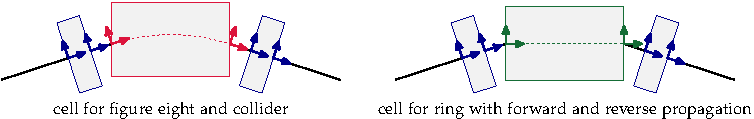
\includegraphics{Layouts/models-00}
  \caption{Basic cells for the three accelerator models.}
  \label{fig:basic.cells}
\end{figure}

\fref[c]{basic.cells} illustrates the two basic cells. We outline
the quadrupoles in blue, the rectangular bend in red, and the
``straight'' bend in green. The black lines indicate the drifts.
The cell with the rectangular bend does not require patching  because the reference frames of
adjacent elements lie on top of one another. The cell with the
``straight'' bend, however, requires patching t because the adjacent drifts have frames that
are rotated with repect to those of the ``straight'' bend.

\index{build\_PSR@\ptc{build\_PSR}!basic ring}
%
The basic ring (see the \ptc{build_PSR} example in \fref{DNA.subrtns}
on \pref{fig:DNA.subrtns}) has ten cells. It has 70~fibres, each pointing
to one of 70~elements. The ring with forward and reverse propagation has
140~fibres pointing to 140~elements.

The figure-eight and the collider each have 140~fibres pointing to
134~elements. In each of those models the upper and lower rings share
the elements at the start of one cell (long drift, quadrupole, short
drift) and the elements at the end of another cell (short drift,
quadrupole, long drift).

\begin{figure}[ht]
  \centering
  %\includegraphics[width=\textwidth]{illustrations/model-tutorial}
  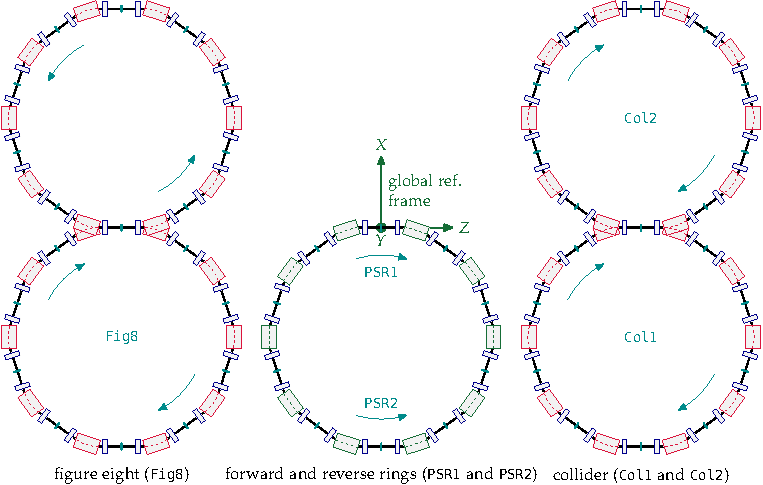
\includegraphics{Layouts/models-01}
  \caption{Accelerator models. Arrows indicate the direction of motion
           of particle beams in the constituent layouts.}
  \label{fig:accel.models}
\end{figure}

Our three tutorial examples are not real accelerators: They do not
have particle injectors or dumps; and two of the examples are not
physically possible, because some of their elements overlap in space.
The goal of these examples is to introduce the principal \PTC\ concepts
involved in modeling the geometry of an accelerator. After learning
these concepts, we can use \PTC\ to model complex real-world
accelerators.


\section{Geometry Tutorial Source File}
\label{sec:geom.tut}

\index{PTC!source file}
\index{source file!geometry tutorial}
\index{geometry!tutorial source file}
\index{ptc\_geometry.f90@\ptc{ptc\_geometry.f90}!geometry tutorial source file}
%
The example code in this chapter is from the \PTC\ geometry tutorial
source file, \ptc{ptc_geometry.f90}, which is given in
\Aref{geom.tutorial}. The line numbers of the code in the examples
refer to the line numbers of the code in that appendix.


\subsection{Initial Code}
\label{sec:init.code}

The initial code in the \ptc{ptc_geometry.f90} source file
includes type declarations and performs some initialization.

\setptclinenums{1}{5}
\begin{ptccode}[
  label={\ptctitle{\ptc{ptc_geometry.f90}\quad\small This program
                   describes the geometry of several \PTC\ lattices.}}
]
program ptc_geometry
use madx_ptc_module
use pointer_lattice
implicit none

logical(lp) :: doit
integer :: i, j, mf, pos, example
real(dp) :: b0
real(dp), dimension(3) :: a, d
real(dp), dimension(6) :: fix1, fix2, mis, x
type(real_8), dimension(6) :: y1, y2
type(layout), pointer :: L1, L2, L3, L4, L5, L6
type(layout), pointer :: PSR1, PSR2, Fig8, Col1, Col2
type(fibre), pointer :: p1, p2, p3, pf, b, f
type(internal_state) :: state

! some simple fitting objects for the fake collider complex
type(pol_block) :: qf(2), qd(2) 
type(normalform) :: n1, n2
type(damap) :: id
type(taylor) :: eq(4)
type(gmap) :: g
!-----------------------------------
!-----------------------------------
    interface
       subroutine build_PSR(PSR)
         use madx_ptc_module
         use pointer_lattice
         implicit none
         type(layout), target :: PSR
       end subroutine build_PSR
       subroutine build_PSR_minus(PSR)
         use madx_ptc_module
         use pointer_lattice
         implicit none
         type(layout), target :: PSR
       end subroutine build_PSR_minus
       subroutine build_Quad_for_Bend(PSR)
         use madx_ptc_module
         use pointer_lattice
         implicit none
         type(layout), target :: PSR
       end subroutine build_Quad_for_Bend
    end interface
!

call ptc_ini_no_append          \label{lin:init.layout}
\end{ptccode}

%\fxnote{What does \ptc{use\_info = .true.} do?!?}

\index{PTC!universe}
\index{universe!PTC}
\index{MAD universe|see{PTC universe}}
\index{global variable!\ptc{m\_u}}
\index{m\_u@\ptc{m\_u}!global variable}
\index{DNA database!\ptc{m\_u} global variable}
\index{module!\ptc{madx\_ptc\_module}}
\index{madx\_ptc\_module@\ptc{madx\_ptc\_module}!module}
\index{linked list!\ptc{m\_u} global variable}
%
\et{The module \ptc{madx_ptc_module}  defines the global variable}
\ptc{m_u}.\label{mad.univ}%
\sidenote{Think "\emph{M}\textsc{ad} \emph{U}niverse".}
This variable, which we shall use frequently, denotes a linked list
of layouts%
\sidenote{We use the linked-list aspect of \ptc{m_u} only briefly
in \STref{DNA.array}.}
that will \et{contain} our \DNA\ database \et{as well as the trackable layouts.} 

%The \ptc{gino}
%mentioned on \lref{gino} refers to a
%Windows$^\text{\textregistered}$-based graphical user
%interface developed for \PTC\ by \'Etienne Forest.
%Its use is not required.

\PTC\ uses the following type declarations for modeling accelerator
topologies:
\begin{itemize}
  \item \ptc{real(dp)} for double precision real numbers,
  \item \ptc{type(layout)} for \ptctyp{layout}s,
  \item \ptc{type(fibre)} for \ptctyp{fibre}s,
  \item \ptc{type(internal_state)} for setting the characteristic
         dynamics desired of your accelerator (see \TAref*{states}).
\end{itemize}
These data types will be discussed in this chapter.

\PTC\ uses the following type declarations for analyzing accelerator
properties \et{through the use of Taylor maps:}
\begin{itemize}
  \item \ptc{type(real_8)} for polymorphs,
  \item \ptc{type(pol_block)} for polymorphic blocks,
  \item \ptc{type(normalform)} for normal forms,
  \item \ptc{type(damap)} for a vector of Taylor maps
        (differential algebra maps),
  \item \ptc{type(taylor)} for single Taylor maps,
  \item \ptc{type(gmap)} for a vector of Taylor maps.
\end{itemize}
These latter data types will be described in \CTref*{polymorphs.knobs}.

\index{global variable!\ptc{lmax}}
\index{lmax@\ptc{lmax}!global variable}
\index{integration node!setting maximum length}
%
%The global variable \ptc{Lmax} defines the maximum length (here
%100~meters!) of an integration node. For more information about
%splitting elements into integration nodes,
%see \TCref*{symplectic.integ}.

%This initial code also, on \lref{init.layout}, initializes a layout;
%this must be done before starting \PTC's
%Gino$^\text{\textregistered}$-based graphical user interface for Windows.


\section{Subroutines}
\label{sec:geom.sub}

\index{DNA sequence!example source code}
\index{DNA database!example source code}
%
The end of the \ptc{ptc\_geometry.f90} source file contains three
subroutines we use to create the \DNA\ sequences---non-trackable
layouts for our \DNA\ database. \fref[c]{DNA.subrtns} shows the
layouts that the three subroutines create. In subsequent sections
of this chapter, we describe how to use the layouts from this database,
or pieces of these layouts, to form the accelerator models of
\fref{accel.models}.

\begin{figure}[ht]
  \centering
  %\includegraphics[width=\linewidth]{illustrations/model-PSR}
  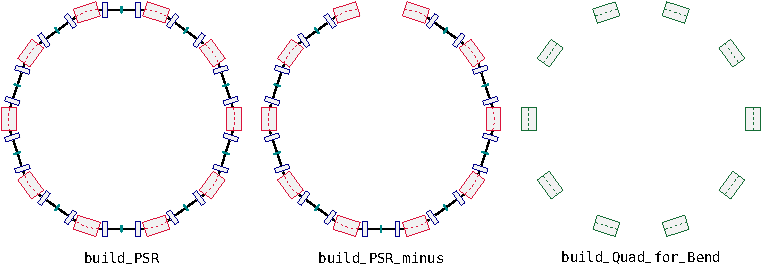
\includegraphics{Layouts/models-02}
  \caption{Subroutines for creating \DNA\ sequences.}
  \label{fig:DNA.subrtns}
\end{figure}


\subsection{build\_PSR}
\label{sec:build.psr}

\index{build\_PSR@\ptc{build\_PSR}!example source code}
%
The subroutine \ptc{build_PSR} creates the basic ten-cell ring
lattice shown on the left in \fref{DNA.subrtns}.

\setptclinenums{532}{5}
\begin{ptccode}
subroutine  build_PSR(PSR)
use run_madx
use pointer_lattice
implicit none

type(layout), target :: PSR

real(dp) :: ang, brho, kd, kf, Larc
type(fibre) :: b, d1, d2, qd, qf
type(layout) :: cell
!-----------------------------------

call make_states(.false.)       \label{lin:bptc.psrstates}
exact_model = .true.
madlength = .false.             \label{lin:eptc.psrstates}

ang = (twopi * 36.d0 / 360.d0)
Larc = 2.54948d0
brho = 1.2d0 * (Larc / ang)
call set_mad(brho = brho, method = 2, step = 10) \label{lin:psr.setmad}
madkind2 = drift_kick_drift

kf =  2.72d0 / brho
kd = -1.92d0 / brho

d1 = drift("D1", 2.28646d0)     \label{lin:bptc.psrlatt}
d2 = drift("D2", 0.45d0)
qf = quadrupole("QF", 0.5d0, kf)
qd = quadrupole("QD", 0.5d0, kd)
b  = rbend("B", Larc, ang) \label{lin:psr.bend}
cell = d1 + qd + d2 + b + d2 + qf + d1 \label{lin:eptc.psrlatt}

PSR = 10 * cell
PSR = .ring.PSR                 \label{lin:psr.ring}

call survey(PSR)                \label{lin:psr.survey}
end subroutine build_PSR
\end{ptccode}

\index{internal states!example source code}
\index{state!internal}
\index{make\_states@\ptc{make\_states}!routine}
\index{routine!\ptc{make\_states}}
\index{exact\_model@\ptc{exact\_model}!global parameter}
\index{global parameter!\ptc{exact\_model}}
\index{madlength@\ptc{madlength}!flag}
\index{flag!\ptc{madlength}}
%
\glossary[ptccmds](make\_states)%
  {make\_states(<\textit{\normalfont{bool}}>)}%
  {This subtoutine sets internal-state variables associated
   with the particle type.
   In particular, use \ptc{call make\_states(true)} for electrons,
   and \ptc{call make\_states(false)} for protons.}
%
The \lref[s]{bptc.psrstates}--\lref*{eptc.psrstates} set important
internal state variables for tracking. In the call to
\ptc{make_states}, the boolean argument \ptc{.false.} means we are
modeling a proton lattice. Use \ptc{.true.} for electrons.%
\sidenote{For other particles, use the ratio of particle mass to
electron mass as the argument of \ptc{make_states}.}
To use the full ``square-root'' Hamiltonian, we set the global
parameter \ptc{exact_model} to \ptc{.true.} 
%
%The global variable
%\ptc{default}, of type \ptctyp{internal_state}, is here modified
%from its default value by adding the following two flags:
%\begin{itemize}
%  \item \ptc{nocavity}, which tells \PTC\ to ignore RF cavities;
%  \item \ptc{exactmis}, which tells \PTC\ to treat misalignments exactly.
%\end{itemize}
%(For more on internal-state variables, see \Aref{states}.)
Finally, we set the flag \ptc{madlength} to \ptc{.false.} This
means that \PTC\ will use the arc length, rather than the chord
length, to define the geometry of a rectangular bending magnet.
Use \ptc{.true.} to make \PTC\ use the chord length. \et{The line \ptc{madkind2 = drift_kick_drift} sets the explicit symplectic integrator to a drift-kick-drift split.}

\begin{marginfigure}\forcerectofloat
  %\includegraphics{illustrations/rbend}
  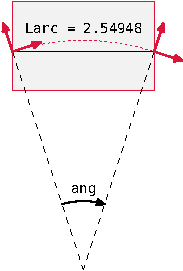
\includegraphics{Layouts/models-04}
  \caption{Geometry of the rectangular bend.}
  \label{fig:rect.bend}
\end{marginfigure}

%\fxnote{Need to say something about \ptc{madkind2}.}

\index{set\_mad@\ptc{set\_mad}!routine}
\index{routine!\ptc{set\_mad}}
\index{integration nodes!specifying number of}
\index{energy!specifying}
%
\makeussubscript
\label{set.mad}
The call, in \lref{psr.setmad}, to \ptc{set\_mad} defines (via
\ptc{brho}) the scale momentum $p_o$ for the fibres in the
layout returned by this subroutine. It also specifies the type
(\ptc{method = 2}) and number (\ptc{STEP = 10}) of integration steps
in the body of each element. We then define the five fibres needed
for our basic cell:
\makeusother
\begin{itemize}
  \item Fibres \ptc{d1} and \ptc{d2} denote the long and short drifts.
  \item Fibres \ptc{qf} and \ptc{qd} denote the focusing and defocusing
        quadrupoles.
  \item And fibre \ptc{b} denotes the rectangular bending magnet.
        Note that it is defined by its arc length and bend angle---here
        \ptc{Larc} and \ptc{ang}, respectively.
        See \fref{rect.bend}.
\end{itemize}
The symbols in quotes (\eg, \ptc{"QF"}) are the \emph{names} given
to these elements.%
\sidenote{Because a layout may have any number of these elements,
the names actually define \emph{classes} of elements.}
We may now define the variable \ptc{cell}, of type \ptctyp{layout}, as
the appropriate sequence of fibres. Finally, the layout \ptc{PSR}
returned by this subroutine is defined as 10 cells, and
\lref{psr.ring} modifies \ptc{PSR} to make it a ring, \ie, closed.

\index{survey@\ptc{survey}!routine}
\index{routine!\ptc{survey}}
%
At this point, \lref{psr.ring}, the elements of the \PSR\ lattice
are present, and in the correct sequence of fibres, in layout
\ptc{PSR}. But should we ask for the location of those elements,%
\sidenote{The way to ask this of \PTC\ will become clear later in
this chapter. See, for example, \pref{move.elem}---especially the
discussion of moving and rotating elements.}
we would discover that all of them have their entrance frames at
the global origin.  In other words, they are all stacked on top
of one another at the global origin.
%\linenumberfrequency{0}
%\begin{ptccode}[frame=none]
%  p => PSR%start
%  do i = 1, PSR%n
%    write(mf,'(a)') p%mag%name
%    write(mf,'(a,3(1x,f13.7))') "a:   ", p%chart%f%a
%  end do
%\end{ptccode}
The call to \ptc{survey} causes \PTC\ to loop through the fibres in
\ptc{PSR}, moving each element so that its entrance frame coincides
with the exit frame of the previous element. For the \PSR\ lattice,
the reference frames for the bends and quadrupoles line up exactly
with those of their adjacent drifts. As a consequence, this lattice
requires no patching. We have therefore finished building the
\PSR\ lattice in \PTC.



\newthought{Some readers will complain} that the set of
\lref[s]{bptc.psrlatt} through \lref*{eptc.psrlatt} violates the
philosophy of \PTC---and they have a point. This may seem subtle,
but we urge all other readers to invest the time required to
comprehend this point. Look, for example, at the definition of the
bend given in \lref{psr.bend}. After careful consideration of this
definition and what happens on the succeeding lines, the reader
should recognize that this definition actually serves a dual purpose.
On the one hand, the setting of arc length and bend angle define the
\emph{geometry} of the element. On the other hand, this line also
serves to define the \emph{physics} of this element. To verify this
claim, query \PTC\ for the magnetic field of this element:
\linenumberfrequency{0}
\begin{ptccode}[frame=none]
  write(6,'(a,f7.4)') "PSR B-field = ", b%mag%bn(1) * brho
\end{ptccode}
\linenumberfrequency{5}
will do the trick. You will learn that \PTC\ already knows the
magnetic field has a value of \SI{1.2}{T}! This information, of
course, requires a knowledge of not only the geometry, but also the
particle mass and energy. \emph{Here} is the apparent violation of
the \PTC\ philosophy, which aims to separate the geometric
description of beamline elements (location, reference frames, \etc)
from their physical content (magnetic field strength, \etc). The
resolution of this conflict lies in the fact that once we have
nailed down the geometry, we are then free to modify the lattice
with misalignments, changes to the magnetic field, and the like.

\et{
\newthought{Some readers, who fully understand the flexibility of PTC,  will most certainly object to \lref{psr.survey}! } 
Indeed the claim is, as the reader will discover soon, that magnets can be placed in any bizarre positions. Then what is the \ptc{survey} command doing?
Forest claimed that he could have chosen to be more ``Catholic than the Pope'' in which case the \ptc{survey} command would not exist.
Indeed one can place magnets ``manually'' and \PTC\ can then compute the necessary patches between them. This is the ``fundamentalist'' view of \PTC . With that philosophy, the survey command is useless.  


Indeed most lattices, or pieces of lattices, come from standard codes. In standard codes the survey command places the magnets using the assumption that no patches are needed between the elements. Therefore a simple sequence like the BMAD sequence \ptc{CELL: LINE=( D1M,SD1,QD,D2,SD2,B,D2,SD2,QF,D1)} already assumes a relative placement of the magnets.

 The reader must realize that the locution ``assumes no patches'' is completely code dependent. \PTC\ and BMAD use the geometry described in the  MAD8
manual from which a ``no patch'' lattice entails a certain relative placement. However, for lattices involving vertical bends, the result will differ from the code SAD of KEK. In the code SAD, the exit frame of a rotated bend will not be lined up with that of a vertically rotated bend in MAD8. Therefore the survey command of SAD will produce a different lattice from MAD, \PTC\ or BMAD. In MAD, the rotation that brings  a dipole off the mid-plane is undone at the exit. In SAD, it  is not so as SAD tries to ``parallel transport'' the frame of reference. 

It is important to realize, in the lens frame work, that the frame of references are really arbitrary. No one can say that SAD is better than MAD or vice versa. \PTC\ adopted the MAD convention simply because Forest collaborated initially with the MAD team. Actually Forest emphasizes this point by stating that he often has the urge to rotate the exit frame of reference of all magnets by some arbitrary angle just to prove this point. 

In reality, it is possible to link \PTC\ with a CAD program and generate an arbitrarily oriented sequence of magnets requiring patches. This is the power of \PTC\ that we try to explain here. 

Ultimately the survey command of \PTC\ has two minor purposes. First, from  purely internal point of view, it insures self-consistency. If a lattice has been patched, then the survey command, which tracks the positions of the lattice through should not ``move'' it. If it does then either patches are missing or badly computed. In any event \PTC\ is in a confused state. Secondly, most people will input into \PTC\ standard lattices and expect the standard survey command  of MAD to ``place'' the magnets in their (relative) correct place. If \PTC\ did not have a survey command, any standard user would scream for it!

But in summary, simply remember that \PTC\ can put the magnets in any arbitrary position and then track the beam. \PTC\ is ideally suited to be incorporated in a CAD program and produce ``instant'' tracking through a complex 3-d geometry.

}
\subsection{build\_PSR\_minus}

\index{build\_PSR\_minus@\ptc{build\_PSR\_minus}!example source code}
%
The subroutine \ptc{build_PSR_minus} defines the partial ring shown
in the center of \fref{DNA.subrtns}. It begins with a bend, a short
drift, a quadrupole, and a long drift; it continues with eight
\PSR\ cells; and it concludes with a long drift, a quadrupole, a short
drift, and a bend. Relative to the \PSR\ lattice, this partial ring is
missing a short drift, a quadrupole, two long drifts, a quadrupole,
and a short drift. The subroutine is a straightforward modification of
that for \ptc{build_PSR}.
%
\fxnote{Actually, this code sets \ptc{method=6} in the call to
\ptc{set\_mad}. Should we change this, or comment on it?}

\linenumberfrequency{5}
\setptclinenums{572}{5}
\begin{ptccode}
subroutine  build_PSR_minus(PSR)
use madx_ptc_module
use pointer_lattice
implicit none

type(layout), target :: PSR

real(dp) :: ang, brho, kd, kf, Larc
type(fibre) :: b, d1, d2, qd, qf
type(layout) :: cell
!-----------------------------------

call make_states(.false.)
exact_model = .true.
madlength = .false.

ang = (twopi * 36.d0 / 360.d0)
Larc = 2.54948d0
brho = 1.2d0 * (Larc / ang)
call set_mad(brho = brho, method = 6, step = 10)
madkind2 = drift_kick_drift

kf =  2.72d0 / brho
kd = -1.92d0 / brho

d1 = drift("D1", 2.28646d0)
d2 = drift("D2", 0.45d0)
qf = quadrupole("QF", 0.5d0, kf)
qd = quadrupole("QD", 0.5d0, kd)
b  = rbend("B", Larc, ang)
cell = d1 + qd + d2 + b + d2 + qf + d1

PSR = b + d2 + qf + d1 + 8 * cell + d1 + qd + d2 + b
PSR = .ring.PSR

call survey(PSR)
end subroutine build_PSR_minus
\end{ptccode}


\subsection{build\_Quad\_for\_Bend}

\index{build\_Quad\_for\_Bend@\ptc{build\_Quad\_for\_Bend}!example source code}
%
The subroutine \ptc{build_Quad_for_Bend} defines the layout shown
on the right in \fref{DNA.subrtns}. It has ten ``straight'' bends,
which have the same length as the rectangular bends in the
\PSR\ lattice. Because the entrance and exit frames of the ``straight''
bends are not rotated, we will need to insert patches everywhere.
These patches will describe both rotations and drifts between the
elements. In fact, because this layout contains no focusing elements,
its entries will be used only in other layouts.

\setptclinenums{612}{5}
\begin{ptccode}
subroutine  build_Quad_for_Bend(PSR)
use run_madx
use pointer_lattice
implicit none

type(layout),target :: PSR

real(dp) :: ang, ang2, brho, b1, Larc, Lq
type(fibre) :: b
!-----------------------------------

call make_states(.false.)
exact_model = .true.
madlength = .false.

ang = (twopi * 36.d0 / 360.d0)
Larc = 2.54948d0
brho = 1.2d0 * (Larc / ang)
call set_mad(brho = brho, method = 6, step = 10)
madkind2 = drift_kick_drift     \label{lin:qfb.same}

ang2 = ang / two                \label{lin:bptc.qfb.bend}
b1 = ang / Larc
Lq = Larc * sin(ang2) / ang2

b = quadrupole("B_QUAD", Lq, 0.d0);
call add(b, 1, 0, b1)           \label{lin:qfb.b1}
b%mag%permfringe = .true.       \label{lin:bptc.qfb.frng}
b%magp%permfringe = .true.
b%mag%p%bend_fringe = .true.
b%magp%p%bend_fringe = .true.   \label{lin:eptc.qfb.bend}

PSR = 10 * b
PSR = .ring.PSR

call survey(PSR)                \label{lin:qfb.survey}
end subroutine build_Quad_for_Bend
\end{ptccode}

Except for some changes in the type declarations, the code through
\lref{qfb.same} in this subroutine is identical to that in the
previous two subroutines. The ``straight'' bend is created in
\lref[s]{bptc.qfb.bend} through \lref*{eptc.qfb.bend}. We first
compute the length \ptc{Lq} as the chord length of the \PSR's
rectangular bend. To achieve the desired ``straight'' reference
frames, we define the ``straight'' bend as a zero-strength
quadrupole. Then, to make this a dipole, we set, in \lref{qfb.b1},
the normalized dipole strength of \ptc{b} to the computed value
\ptc{b1}. Finally, we set some flags to give this magnet the fringe
fields appropriate to a rectangular bend.

Query: After the call to \ptc{survey} in \lref{qfb.survey}, where
in the global frame are the magnets that this subroutine defines?%
\sidenote{They lie all in a straight line, one after the other,
starting at the global origin and extending to a point 10\,\ptc{Lq}
out along the $z$ axis. Making this layout look like the right-hand
layout of \fref{DNA.subrtns} will require more work.}


\section{Populating the \DNA\ Database}
\label{sec:pop.DNA}

\index{DNA database!populating}
\index{DNA sequence!populating DNA database}
\index{layout!non-trackable}
%
Using the subroutines described in the previous section, we shall
populate our \DNA\ database with six \DNA\ sequences (non-trackable
layouts): \ptc{L1}, \ptc{L2}, \ptc{L3}, \ptc{L4}, \ptc{L5}, and
\ptc{L6}. Note that we shall want each element in our three
accelerator models to appear once and only once in the \DNA-sequence
portion of the \DNA\ database. This uniqueness will reflect the
uniqueness of the individual beamline elements in our accelerators.

\index{layout!trackable}
%
Layouts \ptc{L1} and \ptc{L2} will provide the elements for the
concentric rings accelerator: trackable layouts \ptc{PSR1} and
\ptc{PSR2}. (See \fref{accel.models}.) Layouts \ptc{L3} and \ptc{L4}
will provide the elements for the figure-eight accelerator: trackable
layout \ptc{Fig8}. And layouts \ptc{L5} and \ptc{L6} will provide the
elements for the collider: trackable layouts \ptc{COL1} and \ptc{COL2}.
\tref[c]{DNA.dbase} summarizes the layouts we plan to create: six
\DNA\ sequences, or non-trackable layouts, and the five trackable layouts.

\begin{table}[t]
  \caption{DNA database for the \PTC\ geometry tutorial}
  \label{tbl:DNA.dbase}
  \begin{center}
    \begin{tabular}{ll} \toprule
  Non-trackable layouts & Trackable layouts \\ \midrule
  \ptc{L1}: 70 elements (\ptc{build_PSR}) & 
    \ptc{PSR1}: created from \ptc{L1} and \ptc{L2} \\
  \ptc{L2}: 10 elements (\ptc{build_Quad_for_Bend}) & 
    \ptc{PSR2}: created from \ptc{L1} and \ptc{L2} \\
  \ptc{L3}: 64 elements (\ptc{build_PSR_minus}) & 
    \ptc{Fig8}: created from \ptc{L3} and \ptc{L4} \\
  \ptc{L4}: 70 elements (\ptc{build_PSR}) & 
    \ptc{Col1}: created from \ptc{L6} \\
  \ptc{L5}: 64 elements (\ptc{build_PSR_minus}) & 
    \ptc{Col2}: created from \ptc{L5} and \ptc{L6} \\
  \ptc{L6}: 70 elements (\ptc{build_PSR}) & \\ \bottomrule
    \end{tabular}
  \end{center}
\end{table}

Query: As initially constructed (by \ptc{build_PSR}), layouts \ptc{L1},
\ptc{L4}, and \ptc{L6} are identical. So also are layouts \ptc{L3} and
\ptc{L5}. Why don't we avoid this duplication?%
\sidenote{Because we want to be able to modify---move, mispower,
\etc--- the individual elements. We do not want changes made to
\ptc{COL1}, for example, to appear in \ptc{Fig8}. \et{All the elements of the DNA are distinct magnets which must exist independently of each other.} }

\index{append\_empty\_layout@\ptc{append\_empty\_layout}!routine}
\index{routine!\ptc{append\_empty\_layout}}
\index{global variable!\ptc{m\_u}}
\index{m\_u@\ptc{m\_u}!global variable}
%
The following four lines create the first \DNA\ sequence:
%
\setptclinenums{60}{5}
\begin{ptccode}
call append_empty_layout(m_u) ! DNA sequence 1
call set_up(m_u%end)
L1 => m_u%end
call build_PSR(L1); L1%name="L1";
\end{ptccode}
%
The call to \ptc{append_empty_layout} appends an empty layout to
the global linked list of layouts \ptc{m_u}. The layout pointer
\ptc{m_u\%end} points to this empty layout. The second line
initializes this new layout; and the third line makes \ptc{L1} point
to it. Finally, the call to \ptc{build_PSR} populates layout \ptc{L1}
with the 70 elements shown for the \PSR\ in \fref{DNA.subrtns}.

We repeat this process five times for layouts \ptc{L2}, \ptc{L3},
\ptc{L4}, \ptc{L5}, and \ptc{L6}. For \ptc{L2}, we call
\ptc{build_Quad_for_Bend}, which populates that layout with 10~elements
(the ``straight'' bends). For \ptc{L3}, we call \ptc{build_PSR_minus},
which populates that layout with 64 elements. And for \ptc{L4},
\ptc{L5}, and \ptc{L6}, we repeat the calls to \ptc{build_PSR} and
\ptc{build_PSR_minus}.
%
\setptclinenums{65}{5}
\begin{ptccode}
call append_empty_layout(m_u) ! DNA sequence 2
call set_up(m_u%end)
L2 => m_u%end
call  build_Quad_for_Bend(L2); L2%name="L2";

call append_empty_layout(m_u) ! DNA sequence 3
call set_up(m_u%end)
L3 => m_u%end
call build_PSR_minus(L3); L3%name="L3";

call append_empty_layout(m_u) ! DNA sequence 4
call set_up(m_u%end)
L4 => m_u%end
call build_PSR(L4); L4%name="L4";

call append_empty_layout(m_u) ! DNA sequence 5
call set_up(m_u%end)
L5 => m_u%end
call build_PSR_minus(L5); L5%name="L5";

call append_empty_layout(m_u) ! DNA sequence 6
call set_up(m_u%end)
L6 => m_u%end
call build_PSR(L6); L6%name="L6";
\end{ptccode}
%
We now have six \DNA\ sequences, or non-trackable layouts, in our
\DNA\ database. Moreover, each beamline element appears just once
in that database.

\index{doko!described}
\index{element!doko for multiple use}
%
The \PTC\ type \ptctyp{element} contains an object, \ptc{doko}
(from the Japanese word for ``where''), that enables \PTC\ to
keep track of which fibres point to a given beamline element.
This object \ptc{doko} allows \PTC\ to use a given element multiple
times in the database of trackable layouts. We shall see several
examples of this in the next section.



\section{Modeling Complex Accelerator Topologies}
\label{sec:model.topos}

%The next step is to create the trackable layouts.
%When we are done, we will set up the \DNA\ arrays.

\index{accelerator topology!complex}
\index{modeling!accelerator topologies}
\index{layout!trackable}
%
In the previous section, we created the layouts in the left-hand
column of \tref{DNA.dbase}. We now set about creating the
layouts (right-hand column of \tref{DNA.dbase}) for the three
accelerator models shown in \fref{accel.models}: the ring with
forward and reverse propagation, the figure-eight lattice, and
the collider. Complex accelerator topologies typically have a
one-to-many correspondence between some of the beamline elements
(stored in the \DNA\ sequences of the \DNA\ database) and the
fibres in the trackable layouts. By the end of this section, you
should understand how to set up such correspondences.

\et{
In \Sref{model.topo2s} and beyond, we will see an alternative way to store the \DNA\ and trackable layouts.
The \DNA\ will be stored in the  mad_universe \ptc{m_u} while all the trackable will be located in the universe \ptc{m_t}.
It will be possible to scan the universe  \ptc{m_u} with a single pointer. But, in the mean time, let us follow the older way of doing things: a single universe for \DNA\ and trackable layouts.
}

\subsection{Ring with Forward and Reverse Propagation}

\begin{marginfigure}[4\baselineskip] \forceversofloat
  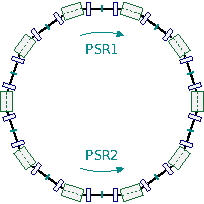
\includegraphics{Layouts/models-05}
  \caption{Ring with forward and reverse propagation.}
  \label{fig:fwd.rev.ring}
\end{marginfigure}

\index{accelerator topology!model of ring with forward and reverse propagation}
\index{ring with forward and reverse propagation!modeling}
\index{forward propagation!example}
\index{backward propagation!example}
%
Here we model an accelerator that carries a pair of
counter-propagating beams (\fref{fwd.rev.ring}, also middle
lattice in \fref{accel.models}). The two beams will propagate
through different layouts---\ptc{PRS1} for the forward-propagating
beam, and \ptc{PRS2} for the backward-propagating beam---but
the two trackable layouts must, of course, share the same ring
with the same beamline elements. They will just have different
directions of propagation and oppositely charged particles.

There is a further complication: this ring uses ``straight'' bends
instead of rectangular bends (see \fref{basic.cells}). In order to
place these elements in their proper locations, we will use the
lattice of layout \ptc{L1} as a guide, taking the ``straight''
bends from layout \ptc{L2}.%
\sidenote{The point of this complication is to illustrate some of
\PTC's geometry operations and the process of patching.
It should also, we hope, emphasize the \LEGO-block concepts of
\PTC\ (\cf\ \fref{LEGO.maps} and the associated discussion).}
The final result will be a pair of layouts, \ptc{PSR1} and
\ptc{PSR2}, each of which refer to fibres in two different
\DNA\ sequences, \ptc{L1} and \ptc{L2}.

\index{append\_empty\_layout@\ptc{append\_empty\_layout}!routine}
\index{routine!\ptc{append\_empty\_layout}}
%
We begin by calling \ptc{append_empty_layout} on \ptc{m\_u} and then
setting the layout pointer \ptc{PSR1} to point to this new layout:
%
\setptclinenums{94}{2}
\begin{ptccode}
!== PSR1 : forward ring  (layout 7)
call append_empty_layout(m_u)
PSR1 => m_u%end
\end{ptccode}
%
We shall populate this layout with a linked list of fibres taken
appropriately from layouts \ptc{L1} and \ptc{L2}. Two fibre
pointers \ptc{p1} and \ptc{p2} will step through these two layouts,
and a third fibre pointer, \ptc{f}, will keep track of our location
in \ptc{PSR1}. Elements taken from \ptc{L1} have the correct
geometric relations, but the ``straight'' bends taken from \ptc{L2}
will have to be moved to their correct locations.

\setptclinenums{98}{5}
\begin{ptccode}
p1 => L1%start
p2 => L2%start
do i = 1, L1%n
  if(p1%mag%name == "B") then
    ! read bends from L2
    call append_point(PSR1, p2)    \label{lin:psr1.append.L2}
    f => PSR1%end                  \label{lin:psr1.bgeom}
    d = p1%chart%f%o - f%chart%f%o \label{lin:psr1.comp.d}
    call translate(f, d)           \label{lin:psr1.trans.d}
    call compute_entrance_angle(f%chart%f%mid, p1%chart%f%mid, a) \label{lin:psr1.comp.a}
    call rotate(f, f%chart%f%o, a, basis = f%chart%f%mid) \label{lin:psr1.egeom}
    p2 => p2%next                  \label{lin:psr1.advance.p2}
  else
    call append_point(PSR1, p1)    \label{lin:psr1.append.L1}
  end if
  p1 => p1%next                    \label{lin:psr1.advance.p1}
end do ! elements in PSR1 now in correct locations
\end{ptccode}

\index{append\_point@\ptc{append\_point}!routine}
\index{routine!\ptc{append\_point}}
%
In the above block of code, we point \ptc{p1} and \ptc{p2}
respectively to the starts of \DNA\ sequences \ptc{L1} and \ptc{L2}.
The \ptc{do} loop over the \ptc{L1\%n} fibres in \ptc{L1} appends
to \ptc{PSR1} the desired fibres from \ptc{L1} or \ptc{L2}---bends
from \ptc{L2}, everything else from \ptc{L1}:
\begin{itemize}
  \item If \ptc{p1} points to a bend, then in \lref{psr1.append.L2}
    we append the current fibre of \ptc{L2} to \ptc{PSR1}. This, of
    course, will always be a ``straight'' bend---a \ptc{B_QUAD}.
    Later, in \lref{psr1.advance.p2}, we advance \ptc{p2} to the next
    fibre in \ptc{L2}.
  \item If \ptc{p1} does \emph{not} point to a bend, then in
    \lref{psr1.append.L1} we append the current fibre of \ptc{L1}
    to \ptc{PSR1}.
  \item In either case, we advance, in \lref{psr1.advance.p1},
    \ptc{p1} to the next fibre in \ptc{L1}.
\end{itemize}

\index{translate@\ptc{translate}!routine}
\index{routine!\ptc{translate}}
\index{compute\_entrance\_angle@\ptc{compute\_entrance\_angle}!routine}
\index{routine!\ptc{compute\_entrance\_angle}}
\index{rotate@\ptc{rotate}!routine}
\index{routine!\ptc{rotate}}
\index{global frame!used to compute local reference frame}
%
After we append a ``straight'' bend to \ptc{PSR1}, we must do
some extra work to place it in the correct location. Since we
want a given ``straight'' bend to have the same location and
orientation as the corresponding rectangular bend, we simply
compute and perform the required translations and rotations.
This happens in \lref[s]{psr1.bgeom} through \lref*{psr1.egeom}:
\label{move.elem}
\begin{enumerate}
  \item Point \ptc{f} to the fibre most recently appended to
    \ptc{PSR1}.
  \item Compute, in \lref{psr1.comp.d}, the vector \ptc{d}
    from the center of the newly appended ``straight'' bend
    (\ptc{f\%chart\%f\%o})%
    \sidenote{Read \ptc{f\%chart\%f\%o} as
    ``\ptc{f}-chart-frame-center''.}
    to the center of the corresponding
    rectangular bend in \ptc{L1} (\ptc{p1\%chart\%f\%o}).
  \item Translate the newly appended fibre (\lref{psr1.trans.d}).
  \item Compute, in \lref{psr1.comp.a}, the rotation \ptc{a}
    from the frame attached to the middle of the newly appended
    ``straight'' bend (\ptc{f\%chart\%f\%mid}) to the frame
    attached to the middle of the corresponding rectangular bend
    in \ptc{L1} (\ptc{p1\%chart\%f\%mid}).%
    \sidenote{Because rotations do not commute, their order is
    important. \PTC\ performs co\"ordinate rotations in the order
    $x$-axis, $-y$-axis, $z$-axis.}
%    Note that \ptc{a} denotes a real three-vector (see
%    \TPref{sec:init.code} \lref{decl.ad}).
  \item Rotate the newly appended fibre about its center
    (\ptc{f\%chart\%f\%o}) by angles \ptc{a}, which are given
    with respect to the frame attached to the middle of that
    element (\ptc{f\%chart\%f\%mid}).
\end{enumerate}

\index{find\_patch@\ptc{find\_patch}!routine}
\index{routine!\ptc{find\_patch}}
\index{patch!inserting}
\index{patching!find\_patch@\ptc{find\_patch} routine}
%
When the above \ptc{do} loop terminates, the beamline elements of
\ptc{PSR1} are all in their correct locations. However (recall the
discussion concerning \fref{basic.cells}) the ``straight'' bends
of \ptc{PSR1} all require patching. This happens in the following
block of code:
%
\setptclinenums{116}{5}
\begin{ptccode}
f => PSR1%start
do i = 1, PSR1%n
  if(f%mag%name == "B_QUAD") then
    call find_patch(f%previous, f, next = .true.)
    call find_patch(f, f%next, next = .false.)
  end if
  f => f%next
end do ! PSR1 now patched
\end{ptccode}
%
Within the \ptc{do} loop over all elements in \ptc{PSR1}, we apply
the patches required between each \ptc{B_QUAD} (or ``straight'' bend)
and its preceding and trailing elements. No other elements require
patching. \et{If a CAD program was linked to \PTC , which would be of great use, then the need for patching would always be there as soon as a magnet is moved. A CAD program would use \PTC\ in its purest and intended form: magnets have no preferential placement. }

Finally, in the following three lines of code, we give layout \ptc{PSR1}
a formal name, and we ensure that it forms a closed topological ring,
so that particles can circulate. Note that the second two lines must
\emph{both} be executed to make the layout \ptc{PSR1} form a closed ring.
The call to \ptc{ring_L} in \lref{psr1.ringL} sets some pointers inside
the layout \ptc{PSR1} that connect the end of \ptc{PSR1} to the start,
and vice versa.
%
\setptclinenums{125}{5}
\begin{ptccode}
PSR1%name = "PSR 1"
PSR1%closed = .true.
call ring_L(PSR1, .true.) ! make it a ring topologically \label{lin:psr1.ringL}
\end{ptccode}

Query: At this point, where in the global frame are the magnets,
the ``straight'' bends, of layout \ptc{L2}?%
\sidenote{\label{sn:geom.L2}%
The geometry operations performed on the bend \ptctyp{fibre}s of
\ptc{PSR1} applied, ultimately, to the \ptctyp{element}s in \ptc{L2}.
Hence those elements are now oriented as in the right-hand layout of
\fref{DNA.subrtns}, with the global origin centered between the
adjacent ends of the top two magnets.}

To construct layout \ptc{PSR2} for the backward-propagating beam,
we follow essentially the same steps as for \ptc{PSR1}. (See the
next block of code.) There are three significant differences:
(i) In this case, all the elements are already in their proper
physical locations,${}^\text{\ref{sn:geom.L2}}$ so here we may
omit the geometric computations
and operations performed during the construction of \ptc{PSR1}.
(ii) Because of the backwards propagation, we initialize the
pointers \ptc{p1} and \ptc{p2} respectively to the \emph{ends} of
layouts \ptc{L1} and \ptc{L2}; and we advance those pointers not
to the next but to the \emph{previous} fibres in their respective
layouts. (See \lref[s]{psr2.prev2} and \lref*{psr2.prev1}.)
(iii) We must add the information that the beam described by this
layout traverses its elements in the reverse direction
(\lref{psr2.opp.dir}) and has particles with negative charge
(\lref{psr2.opp.chg}).%
\sidenote{Both direction and charge are properties of fibres,
and both default to +1.}
%
\setptclinenums{129}{5}
\begin{ptccode}
!== PSR2 : backward ring (layout 8)
call append_empty_layout(m_u)
PSR2 => m_u%end

p1 => L1%end
p2 => L2%end
do i = 1, L1%n
  if(p1%mag%name == "B") then
    call append_point(PSR2, p2)
    p2 => p2%previous            \label{lin:psr2.prev2}
  else
    call append_point(PSR2, p1)
  end if
  f => PSR2%end
  f%dir = -1                     \label{lin:psr2.opp.dir}
  f%charge = -1                  \label{lin:psr2.opp.chg}
  p1 => p1%previous              \label{lin:psr2.prev1}
end do

f => PSR2%start
do i = 1, PSR2%n
  if(f%mag%name == "B_QUAD") then
    call find_patch(f%previous, f, next = .true.)
    call find_patch(f, f%next, next = .false.)
  end if
  f => f%next
end do

PSR2%name = "PSR 2"
PSR2%closed = .true.
call ring_L(PSR2, .true.) ! make it a ring topologically
\end{ptccode}

Trackable layouts \ptc{PSR1} and \ptc{PSR2} are now complete.
Both contain 70 fibres pointing to the same set of 70 elements
in \DNA\ sequences \ptc{L1} and \ptc{L2}.


\subsection{Figure-Eight}

\index{accelerator topology!model of figure eight}
\index{figure-eight accelerator!modeling}
%
Here we model a figure-eight lattice---the left-hand lattice in
\fref{accel.models}. It carries a single beam clockwise (forward)
around the lower ring, then counter-clockwise (backward) around
the upper ring. The two rings share several elements in one
straight section. See \fref{accel.fig8}. The single trackable
layout \ptc{Fig8} we shall construct from \DNA\ sequences \ptc{L3}
and \ptc{L4} (see \tref{DNA.dbase}). For the lower ring, we use
the full ten-cell \PSR\ lattice in layout \ptc{L4}. For the upper
ring, we use all of layout \ptc{L3} (\ptc{PRS_minus}), and we
re-use six of the fibres in layout \ptc{L4}. In addition, so that
this layout does not overlap our previous layouts, \ptc{PSR1} and
\ptc{PSR2}, we shall place it \SI{40}{m} distant in the negative~$z$
direction.

\begin{figure}[ht]
  \centering
  %\includegraphics{illustrations/model-fig8}
  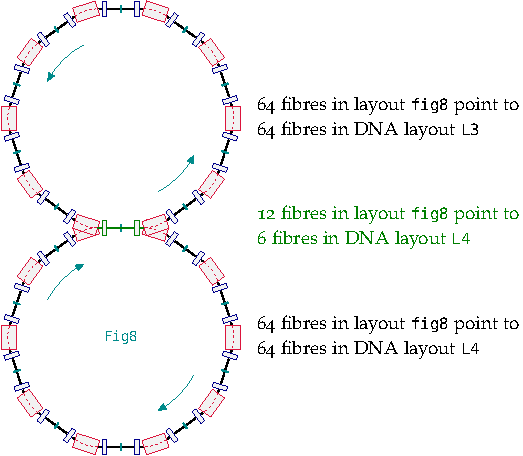
\includegraphics{Layouts/models-03}
  \caption{\ptc{Fig8} fibres pointing to elements in \ptc{L3}
           and \ptc{L4}.}
  \label{fig:accel.fig8}
\end{figure}

The construction of layout \ptc{Fig8} takes place in the following
six blocks of code. We describe each in detail.

\index{global frame!positioning first element in trackable layout}
\index{rotate@\ptc{rotate}!routine}
\index{routine!\ptc{rotate}}
%
In this first block of code, we translate layout \ptc{L4} a
distance \SI{40}{m} in the negative~$z$ direction
(\lref[s]{fig8.btr4}--\lref*{fig8.etr4}).
We then (\lref[s]{fig8.brot}--\lref*{fig8.erot}) rotate layout
\ptc{L3} \ang{180} about the entrance of its first element
(\ptc{L3\%start\%chart\%f\%a}). This rotates the gap in \ptc{L3}
down to the bottom. Now note that the bend to the right of this
gap (after the rotation) belongs to the last fibre in \ptc{L3}.
To finish placing \ptc{L3} in the correct location, we want the
\emph{end} of its last bend to coincide with the entrance of the
first bend in the lower ring, \ptc{L4}. See \fref{ring.match}.
We therefore point, in \lref{fig8.mvp1}, the fibre pointer
\ptc{p1} to the first bend (\ptc{"B"}) in \ptc{L4}; compute, in
\lref{fig8.comp.d}, the vector \ptc{d} from the exit of the last
bend in \ptc{L3} (\ptc{L3\%end\%chart\%f\%b}) to the entrance of
the first bend in \ptc{L4} (\ptc{p1\%chart\%f\%a}); and then
translate, in \lref{fig8.tr3}, layout \ptc{L3} by vector \ptc{d}.
%
\setptclinenums{162}{5}
\begin{ptccode}
!== Fig8 : figure-eight lattice (layout 9)
d = zero                                \label{lin:fig8.btr4}
d(3) = -40.d0
call translate(L4, d)                   \label{lin:fig8.etr4}
a = zero                                \label{lin:fig8.brot}
a(2) = pi
call rotate(L3, L3%start%chart%f%a, a)  \label{lin:fig8.erot}
call move_to(L4, p1, "B", pos)          \label{lin:fig8.mvp1}
d = p1%chart%f%a - L3%end%chart%f%b     \label{lin:fig8.comp.d}
call translate(L3, d)                   \label{lin:fig8.tr3}
\end{ptccode}
%
At this point, the beamline elements for the figure-eight lattice
are all correctly located and oriented.



\index{append\_empty\_layout@\ptc{append\_empty\_layout}!routine}
\index{routine!\ptc{append\_empty\_layout}}
%
In the next block of code, we first call \ptc{append_empty_layout}
on \ptc{m_u} and set the layout pointer \ptc{Fig8} to point to this
new layout. Then, in \lref[s]{fig8.bapp.L4}--\lref*{fig8.eapp.L4},
we append in order all the fibres of \ptc{L4} to \ptc{Fig8}.
%
\setptclinenums{173}{5}
\begin{ptccode}
call append_empty_layout(m_u)
Fig8 => m_u%end
p1 => L4%start                 \label{lin:fig8.bapp.L4}
do i = 1, L4%n
  call append_point(Fig8, p1)
  p1 => p1%next                \label{lin:fig8.p1next}
end do                         \label{lin:fig8.eapp.L4}
\end{ptccode}
%
\begin{marginfigure}[-29\baselineskip]\forceversofloat
  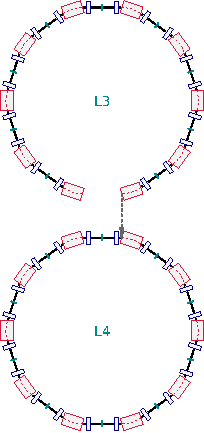
\includegraphics{Layouts/models-06}
  \caption{Matching \ptc{L3} to \ptc{L4}.}
  \label{fig:ring.match}
\end{marginfigure}
We now have the complete lower ring.

\index{append\_point@\ptc{append\_point}!routine}
\index{routine!\ptc{append\_point}}
\index{doko!described}
%
In the next block of code, we start to include the upper ring by
appending to \ptc{Fig8} the first three fibres of the lower ring.
These three new fibres in \ptc{Fig8} will, of course, point to the
same physical elements as do the first three fibres in \ptc{Fig8}:
a long drift, a defocusing quadrupole, and a short drift. During
the calls to \ptc{append_point}, \PTC\ will add this information
to the \ptc{doko}s of the corresponding elements in \ptc{L4}. As a
consequence, each of those three elements in \DNA\ sequence \ptc{L4}
knows that it is pointed to by two different fibres in trackable
layout \ptc{Fig8}.%
\sidenote{Each of those elements already knows it belongs to a
fibre in layout \ptc{L4}.}



Note that we need not initialize the pointer \ptc{p1} to \ptc{L4\%start}: the last execution, in \lref{fig8.p1next}, of \ptc{p1 => p1\%next} returns \ptc{p1} to the beginning of the layout.
%
\setptclinenums{181}{5}
\begin{ptccode}
call append_point(Fig8, p1)
p1 => p1%next
call append_point(Fig8, p1)
p1 => p1%next
call append_point(Fig8, p1)
\end{ptccode}

In the next block of code, we append the fibres of layout \ptc{L3}
to \ptc{Fig8}. Since our beam traverses \ptc{L3} in the reverse
direction, we initialize the fibre pointer \ptc{p1} to \ptc{L3\%end}
(\lref{fig8.p1.set1}), and we advance that pointer to the
\emph{previous} fibre (\lref{fig8.prev1}). During this process,
we take care of two other tasks: We tell \PTC\ that these elements
are traversed in the reverse direction (\lref{fig8.opp.dir}); and,
if the element is a bend, we reverse the sign of the magnetic field
(\lref{fig8.revb}). The particle charge remains the same (default
value +1).
%
\setptclinenums{169}{5}
\begin{ptccode}
p1 => L3%end                   \label{lin:fig8.p1.set1}
do i = 1, L3%n
  call append_point(Fig8, p1)
  Fig8%end%dir = -1            \label{lin:fig8.opp.dir}
  if(p1%mag%name == "B") p1%mag%bn(1) = -p1%mag%bn(1) \label{lin:fig8.revb}
  p1 => p1%previous            \label{lin:fig8.prev1}
end do
\end{ptccode}

\index{doko!described}
%
To complete the upper ring, and hence our trackable layout
\ptc{Fig8}, three fibres remain to be appended: the last three
fibres of the lower ring, \ptc{L4}. This is accomplished in the
next block of code. First, in \lref{fig8.p1.set2}, we point
\ptc{p1} to the fibre containing the short drift near the end of
layout \ptc{L4}. We then append to \ptc{Fig8} that fibre and the
next two. During the calls to \ptc{append_point}, \PTC\ will add
the appropriate information to the \ptc{doko}s of the corresponding
elements.
%
\setptclinenums{195}{5}
\begin{ptccode}
p1 => L4%end%previous%previous  \label{lin:fig8.p1.set2}
call append_point(Fig8, p1)
p1 => p1%next
call append_point(Fig8, p1)
p1 => p1%next
call append_point(Fig8, p1)
\end{ptccode}

\index{check\_need\_patch@\ptc{check\_need\_patch}!routine}
\index{routine!\ptc{check\_need\_patch}}
\index{find\_patch@\ptc{find\_patch}!routine}
\index{routine!\ptc{find\_patch}}
\index{patch!inserting}
\index{patch!checking whether needed}
\index{patching!\ptc{find\_patch} routine}
\index{patching!\ptc{check\_need\_patch} routine}
%
Finally, in the last block of code for \ptc{Fig8}, we give our new
layout a formal name (\ptc{"Figure-Eight"}), ensure that it is
topologically closed, and apply any necessary patches. The call to
\ptc{check_need_patch}, \lref{fig8.chk.patch}, returns the integer
\ptc{pos} equal to zero if no patch is needed. A non-zero value
indicates the type of patch required. By using \ptc{check_need_patch},
we can apply patches only where necessary. Our figure-eight lattice
requires patching because some of the constituent elements are
traversed in the reverse direction. In particular, there are adjacent
fibres \ptc{f} which have opposite values of \ptc{f\%dir}. This
happens between the short drift at end of the common straight section
and the first bend of the upper ring; and also between the last bend
of the upper ring and the subsequent short drift.
%
\setptclinenums{202}{5}
\begin{ptccode}
Fig8%name = "Figure-Eight"
Fig8%closed = .true.
call ring_L(Fig8, .true.) ! make it topologically closed

p1 => Fig8%start
do i = 1, Fig8%n
  call check_need_patch(p1, p1%next, 1.d-10, pos)  \label{lin:fig8.chk.patch}
  if(pos /= 0) call find_patch(p1, p1%next, next = .false.)
  p1 => p1%next
end do
\end{ptccode}

Trackable layout \ptc{Fig8} is now complete. It has 140~fibres
pointing to 134~elements in \DNA\ sequences \ptc{L4} and \ptc{L3}.
Twelve of the fibres in \ptc{Fig8} point to the six elements (four
drifts and two quadrupoles at the top of \ptc{L4}) which are common
to the upper and lower rings. See \fref{accel.fig8}.

\et{There is an interesting anecdote concerning the \PTC\ model of the LHC by Forest and Schmidt. Forest connected the injection line of LHC2 to LHC2 itself. This required a tiny angle due to the kicker at the end of the injection line. However since the injection line had been designed  using forward propagators and the LHC2 is made of backwards propagators, patching also requires a rotation of 180 degrees. Forest was asked, during his presentation, if he had not forgotten to put that rotation. His answer was simply: ``Let us see if \PTC\ has put it.''  Indeed examination of the flat file showed that  \PTC\ had correctly identified the need for a patch. In MADX, the user must on his own, through unreliable brain power, realize that a rotation of 180 degrees is needed to bring the outward horizontal direction of one beam line into what appears to be an inward $x$-direction: look at the common area of the Figure-Eight or the collider.  }


\subsection{Collider}


\index{accelerator topology!model of collider}
\index{collider!modeling}
%
Here we model a collider---\fref{col1.col2}, also the right-hand
lattice in \fref{accel.models}---which has clockwise propagating
beams in each of its two rings. This model comprises two layouts,
\ptc{Col1} and \ptc{Col2}, which we shall construct from
\DNA\ sequences \ptc{L5} and \ptc{L6} (see \tref{DNA.dbase}). For
the lower ring, we use the full ten-cell \PSR\ lattice in layout
\ptc{L6}. For the upper ring, we use all of layout \ptc{L5}
(\ptc{PRS_minus}), and we re-use six of the fibres in layout
\ptc{L6}.%
\sidenote{Yes, this sounds much like the description for layout
\ptc{Fig8}. Be sure to note the \emph{differences}.}
In addition, so that this layout does not overlap our previous
layouts, \ptc{PSR1}, \ptc{PSR2}, and \ptc{Fig8}, we shall place
it \SI{40}{m} distant in the positive~$z$ direction.

The construction of layouts \ptc{Col1} and \ptc{Col2} takes place
in the following four blocks of code. We describe each in detail.

\begin{marginfigure}
  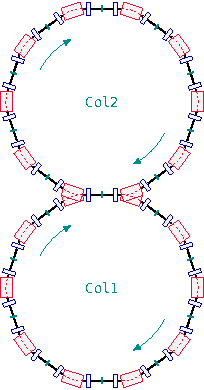
\includegraphics{Layouts/models-07}
  \caption{Collider.}
  \label{fig:col1.col2}
\end{marginfigure}

In this first block of code, we place all the beamline elements of
layouts \ptc{Col1} and \ptc{Col2} in their correct locations: We
translate layout \ptc{L6} a distance \SI{40}{m} in the positive~$z$
direction. We then rotate layout \ptc{L5} \ang{180} about the
entrance of its first element (\ptc{L5\%start\%chart\%f\%a}). This
rotates the gap in \ptc{L5} down to the bottom. To finish placing
\ptc{L5} in the correct location, we want the \emph{end} of its
last bend to coincide with the entrance of the first bend in the
lower ring, \ptc{L6}. We therefore point layout pointer \ptc{p1}
to the first bend (\ptc{"B"}) in \ptc{L6}; compute the vector
\ptc{d} from the exit of the last bend in \ptc{L5}
(\ptc{L5\%end\%chart\%f\%b}) to the entrance of the first bend in
\ptc{L6} (\ptc{p1\%chart\%f\%a}); and then translate layout \ptc{L5}
by that vector \ptc{d}.
%
\setptclinenums{213}{5}
\begin{ptccode}
!== Col1 : lower collider ring (layout 10)
!== Col2 : upper collider ring (layout 11)
d = zero
d(3) = 40.d0
call translate(L6, d)
a = zero
a(2) = pi
call rotate(L5, L5%start%chart%f%a, a)
call move_to(L6, p1, "B", pos)
d = p1%chart%f%a - L5%end%chart%f%b
call translate(L5, d)
\end{ptccode}

\index{append\_empty\_layout@\ptc{append\_empty\_layout}!routine}
\index{routine!\ptc{append\_empty\_layout}}
\index{append\_point@\ptc{append\_point}!routine}
\index{routine!\ptc{append\_point}}
%
In the next block of code, we construct layout \ptc{Col1}: We
call \ptc{append_empty_layout} on \ptc{m_u} and set the layout
pointer \ptc{Col1} to point to this new layout. Then we append
in order all the fibres of \ptc{L6} to \ptc{Col1}. Finally, we
give our new layout a formal name (\ptc{"Collider 1"}) and ensure
that it is topologically closed. This layout does not require
patching.
%
\setptclinenums{225}{5}
\begin{ptccode}
call append_empty_layout(m_u)
Col1 => m_u%end
p1 => L6%start
do i = 1, L6%n
  call append_point(Col1, p1)
  p1 => p1%next
end do

Col1%name = "Collider 1"
Col1%closed = .true.
call ring_L(Col1, .true.) ! make it a ring topologically
\end{ptccode}

In the next block of code, we construct layout \ptc{Col2}: We call
\ptc{append_empty_layout} again on \ptc{m_u}, set the layout
pointer \ptc{Col2} to point to this new layout, and then locate,
in \lref{col2.next.next}, the first short drift in layout \ptc{L6}.
To populate \ptc{Col2}, we now, in
\lref[s]{col2.bapp.str}--\lref*{col2.eapp.str}, march backwards
appending the six elements in the straight section at the top of
layout \ptc{L6} (short drift, defocusing quadrupole, two long drifts,
focusing quadrupole, and short drift). While doing this, we inform
\PTC, in \lref{col2.opp.dir}, that this layout traverses those
elements in the opposite direction. Finally, in
\lref[s]{col2.bapp.L5}--\lref*{col2.eapp.L5}, we append in order all
the fibres of \ptc{L5} to \ptc{Col2}.
%
\setptclinenums{237}{5}
\begin{ptccode}
call append_empty_layout(m_u)
Col2 => m_u%end
p1 => L6%start%next%next    \label{lin:col2.next.next}
do i = 1, 6                 \label{lin:col2.bapp.str}
  call append_point(Col2, p1)
  Col2%end%dir = -1         \label{lin:col2.opp.dir}
  p1 => p1%previous
end do                      \label{lin:col2.eapp.str}
p1 => L5%start              \label{lin:col2.bapp.L5}
do i = 1, L5%n
  call append_point(Col2, p1)
  p1 => p1%next
end do                      \label{lin:col2.eapp.L5}
\end{ptccode}

\index{check\_need\_patch@\ptc{check\_need\_patch}!routine}
\index{routine!\ptc{check\_need\_patch}}
\index{find\_patch@\ptc{find\_patch}!routine}
\index{routine!\ptc{find\_patch}}
\index{patch!inserting}
\index{patch!checking whether needed}
\index{patching!\ptc{find\_patch} routine}
\index{patching!\ptc{check\_need\_patch} routine}
%
In this last block of code for \ptc{Col2}, we give our new layout a
formal name (\ptc{"Collider 2"}), ensure that it is topologically
closed, and apply any necessary patches. This layout requires patches
only where \ptctyp{fibre}\ptc{\%dir} switches sign. As in our earlier
layout \ptc{Fig8}, this happens at the two ends of the common straight
section, where they join the bends of the upper ring.
%
\setptclinenums{251}{5}
\begin{ptccode}
Col2%name = "Collider 2"
Col2%closed = .true.
call ring_L(Col2, .true.) ! make it a ring topologically

p1 => Col2%start
do i = 1, Col2%n
  call check_need_patch(p1, p1%next, 1.d-10, pos)
  if(pos /= 0) call find_patch(p1, p1%next, next = .false.)
  p1 => p1%next
end do
\end{ptccode}

The trackable layouts \ptc{Col1} and \ptc{Col2} are now complete.
They have 140 fibres pointing to 134 elements in \DNA\ sequences
\ptc{L6} and \ptc{L5}. Twelve of the fibres in \ptc{Col1} and
\ptc{Col2} point to the six elements which are common to the upper
and lower rings.


\section{DNA Arrays}
\label{sec:DNA.array}

\index{DNA array!described}
\index{layout!trackable}
\index{DNA database!storing trackable layouts}
\index{allocate@\ptc{allocate}!routine}
\index{routine!\ptc{allocate}}
%
The following code constitutes a bit of housekeeping. We have created a set of six layouts---\ptc{L1}--\ptc{L6}---that form the core of our \DNA\ database. What we do here is tell each of the trackable layouts we have created---\ptc{PSR1}, \ptc{PSR2}, \ptc{Fig8}, \ptc{Col1}, and \ptc{Col2}---which \DNA\ sequences they use. This information is stored in the array \ptc{DNA} that is part of the data held in each \PTC\ \ptctyp{layout}.

In \lref{dna.L1} we record in \ptc{PSR1} the fact that \DNA\ sequence \ptc{L1} is used by \ptc{PSR1}. Then \lref{dna.L2} records the fact that \ptc{PSR1} also uses \DNA\ sequence \ptc{L2}. Note that this latter line makes use of the linked-list character of our \DNA\ database. (Recall, see \pref{mad.univ}, that \ptc{m_u} is a linked list of layouts.) Since \ptc{PSR1\%DNA(1)\%L} already points to \ptc{L1} (see \lref{dna.L1}), and since \ptc{L2} is the next layout in the \DNA\ database, then \ptc{PSR1\%DNA(1)\%L\%next} points to \ptc{L2}. (In this very simple case you could, of course, replace \lref[s]{dna.bdo}--\lref*{dna.edo} with the single statement \ptc{PSR1\%DNA(2)\%L => L2}.) The remaining lines in this block of code populate the \DNA\ arrays for the other trackable layouts.
%
\setptclinenums{267}{5}
\begin{ptccode}
allocate(PSR1%DNA(2))
PSR1%DNA(1)%L => L1                           \label{lin:dna.L1}
do i = 2, 2                                   \label{lin:dna.bdo}
  PSR1%DNA(i)%L => PSR1%DNA(i-1)%L%next ! L2  \label{lin:dna.L2}
end do                                        \label{lin:dna.edo}

allocate(PSR2%DNA(2))
PSR2%DNA(1)%L => L1
do i = 2, 2
  PSR2%DNA(i)%L => PSR2%DNA(i-1)%L%next ! L2
end do

allocate(Fig8%DNA(2))
Fig8%DNA(1)%L => L3
do i = 2, 2
  Fig8%DNA(i)%L => Fig8%DNA(i-1)%L%next ! L4
end do

allocate(Col1%DNA(2))
Col1%DNA(1)%L => L5
do i = 2, 2
  Col1%DNA(i)%L => Col1%DNA(i-1)%L%next ! L6
end do

allocate(Col2%DNA(2))
Col2%DNA(1)%L => L5
do i = 2, 2
  Col2%DNA(i)%L => Col2%DNA(i-1)%L%next ! L6
end do
\end{ptccode}

{
\color{etcol} 

\section{Modeling Complex Accelerator Topologies with two ``MAD universes''}
\label{sec:model.topo2s}



The program \ptc{new_ptc_geometry.f90} is very similar to the program we just examined. \DNA\ or databased layouts are created in the same manner; trackable layouts are also created identically as far as the process is concerned. The main difference is in the storage of these objects. The database layouts are stored in the database universe \ptc{m_u}. The trackable layout are stored in the trackable universe \ptc{m_t}. With this setup we could dispense with the \DNA\ pointers described in the previous section, although they might still be very useful.

To explain this process, we created a new program \ptc{new_ptc_geometry.f90} that contains purposely some empty lines so that the line numbers align perfectly with \ptc{ptc_geometry.f90}. In doing so, we facilitate comparison. The \DNA\ pointers are left in the code since they are used in the fitting example.t

As we will see, the database universe \ptc{m_u} contains all the necessary information and can be scanned as a single linked list irrespective of the number of layouts it happens to contain.

\setptclinenums{1}{5}
\begin{ptccode}[
  label={\ptctitle{\ptc{new_ptc_geometry.f90}\quad\small This program
                   describes the geometry of several \PTC\ lattices using two ``MAD universes.''}}
]
program new_ptc_geometry
use madx_ptc_module
use pointer_lattice
implicit none

logical(lp) :: doit
integer :: i, j, mf, pos, example,poss
real(dp) :: b0
real(dp), dimension(3) :: a, d
real(dp), dimension(6) :: fix1, fix2, mis, x
type(real_8), dimension(6) :: y1, y2
type(layout), pointer :: L1, L2, L3, L4, L5, L6
type(layout), pointer :: PSR1, PSR2, Fig8, Col1, Col2
type(fibre), pointer :: p1, p2, b, f
type(internal_state) :: state
type(fibre_appearance), pointer :: next_doko
! some simple fitting objects for the fake collider complex
type(pol_block) :: qf(2), qd(2)
type(normalform) :: n1, n2
type(damap) :: id
type(taylor) :: eq(4)
type(gmap) :: g
!-----------------------------------
!-----------------------------------
    interface
       subroutine build_PSR(PSR)
         use madx_ptc_module
         use pointer_lattice
         implicit none
         type(layout), target :: PSR
       end subroutine build_PSR
       subroutine build_Quad_for_Bend_New(PSR)
         use madx_ptc_module
         use pointer_lattice
         implicit none
         type(layout), target :: PSR
       end subroutine build_Quad_for_Bend_New
       subroutine build_PSR_minus(PSR)
         use madx_ptc_module
         use pointer_lattice
         implicit none
         type(layout), target :: PSR
       end subroutine build_PSR_minus
    end interface

call ptc_ini_no_append \label{lin:init.layout2}
write(6,*) "Do you want to read an accelerator complex ? yes=1 "  \label{lin:read:uni1}
read(5,*) poss
if(poss==1) then
 call read_universe_database(m_u,'m_u.txt',arpent=my_false)
 call read_universe_pointed(M_u,M_t,'m_t.txt')
 call create_dna(M_u,m_t)
 goto 999
end if  \label{lin:read:uni2}
\end{ptccode}

The first major difference is the possibility of reading the full accelerator complex if it has been produced previously and printed out. 
The commands are found between \lref[s]{read:uni1} through \lref*{read:uni2}. 

All the layouts of the \DNA\ are loaded in the database universe \ptc{m_u} just as before. The major difference is that the trackable layouts are then created into the universe \ptc{m_t} rather than being appended to \ptc{m_u}..

 
{\scriptsize
\setptclinenums{94}{5}
\begin{ptccode}
!== PSR1 : forward ring  (layout 7)                       !== PSR1 : forward ring  (layout 1 of m_t)   \label{lin:dif:1}
call append_empty_layout(m_u)                             call append_empty_layout(m_t) \label{lin:dif:2}
PSR1 => m_u%end                                           PSR1 => m_t%end    \label{lin:dif:3}

p1 => L1%start                                                      
p2 => L2%start                                                      
do i = 1, L1%n                                                      
  if(p1%mag%name == "B") then                                       
    ! read bends from L2                                            
    call append_point(PSR1, p2)                                     
\end{ptccode}
}

This trivial difference is shown on \lref[s]{dif:2} and \lref*{dif:3}. The left hand side shows the original code where the first trackable layout \ptc{PSR1}  is appended at the end the universe \ptc{m_u}; therefore all trackable layouts will follow the database layouts.  On the right hand side, extracted from the program \ptc{new_ptc_geometry.f90}, the first  trackable \ptc{PSR1} is put in the universe \ptc{m_t}. The creation of the other trackable layouts follows the same pattern as \ptc{PSR1}.

With these two universes, the location of trackable and database layouts is unambiguous. Irrespective of their order of creation, all \DNA\ will be sequentially located in \ptc{m_u} and all trackable will be in \ptc{m_t}.

 
\section{Tying a Universe}
\label{sec:model.tie}

As before we can certainly construct the \DNA\ pointers. That still works. However because all the \DNA\ layouts  are in the same universe, it is useful to be able to scan that entire structure as one long link list of fibres. This is explore at the end of the program \ptc{new_ptc_geometry.f90}:

 
{ 
\setptclinenums{524}{5}
\begin{ptccode}
call kanalnummer(mf,"doko.txt")
call TIE_MAD_UNIVERSE(m_u)    \label{lin:tie:uni}
p1=>m_u%start%start
do i=1,m_u%nf  \label{lin:tie:do}
 write(mf,'(i4,1x,a16)') i,p1%mag%name
 next_doko=>p1%mag%doko
  do while(associated(next_doko))
   write(mf,'(a120)') next_doko%parent_fibre%parent_layout%name  \label{lin:lay:nam}
   p2=>next_doko%parent_fibre
   next_doko=>next_doko%next  \label{lin:lay:namn}
 enddo
 p1=>p1%n
end do
close(mf)

call ptc_end(graphics_maybe=2,flat_file=.true.)  \label{lin:ptc:end}
                                  
\end{ptccode}
}

The above piece of code does not do much beside illustrating the structure  of \PTC . First of all, at \lref{tie:uni}, the universe \ptc{\m_u} is ``tied,'' that is to say that a link list connects all the fibres of this universe. The pointers are \ptc{fibre\%p} and \ptc{fibre\%n} for the previous and next fibre respectively. These pointers are nullified if the universe is not tied. They should not be confused with the more important pointers \ptc{fibre\%previous} and \ptc{fibre\%next}  which are the links within a layout and are a quintessential part of \PTC .

The do-loop starting at \lref{tie:do}, scans the entire universe and locates all the occurrences of each magnet. Conversely one could scan a given trackable and check if the magnet is shared. This type of access to the magnets, fibres and layouts can be used in fitting routines to identify where a magnet is.

The result of this loop is printed in file \ptc{doko.txt}. Here is a little bit of that file:

{ 
\setptclinenums{1}{5}
\begin{ptccode}
     .
     .
     .
  66 D2              
PSR 1                                                                                                                   
PSR 2                                                                                                                   
  67 B           \label{lin:b:nil}     
  68 D2             
PSR 1                                                                                                                   
PSR 2                                                                                                                   
  69 QF         \label{lin:qf:psr}      
PSR 1                                                                                                                   
PSR 2                                                                                                                   
  70 D1              
PSR 1                                                                                                                   
PSR 2                                                                                                                   
  71 B_QUAD      \label{lin:b:q}         
PSR 1                                                                                                                   
PSR 2                                                                                                                   
  72 B_QUAD          
PSR 1                                                                                                                   
PSR 2                                                                                                                   
     .
     .
     .

 146 QD           \label{lin:qd:8}        
Figure-Eight                                                                                                            
Figure-Eight                                                                                                            
 147 D2              
Figure-Eight                                                                                                            
Figure-Eight                                                                                                            
 148 B               
Figure-Eight                                                                                                            
 149 D2              
Figure-Eight                                                                                                            
     .
     .
     .
\end{ptccode}
}


We first notice \lref{qf:psr}: it tells us that the quadrupole \ptc{QF} belongs to two objects:  \ptc{PSR1} and \ptc{PSR2}. Thus we are dealing most likely with a collider or some pretzel structure. In a huge object like the LHC, many magnets of the IR (interaction region) are shared between \ptc{LHC1} and \ptc{LHC2}.

On line \lref{qd:8} we see the ``opposite'' case: the same magnet appears twice in the beam line: this is the case of the common section of a ``figure 8'' lattice or a ``dog bone'' structure. This type of situation also appears in recirculators. 

Now we come to ``forensic'' evidence of our weird construction. \ptc{PSR1} and \ptc{PSR2} make a fake ``pretzel'', i.e., the same ring traversed in opposite direction. On  page \pageref{lin:psr1.append.L2} we explained how  the \DNA\ lattice \ptc{L1} creates the database for this pretzel. However, to show the power of patching, we replaced the normal dipole \ptc{B} (of \lref{b:nil}) by the straight elements of layout \ptc{L2}, namely the ten quadrupoles \ptc{B_QUAD}.

For convenience in the creation of this object, the original elements \ptc{B}, which are elements of \ptc{L1},  are never used in the final trackable lattices of \ptc{m_t}. Therefore there are no layouts using \ptc{B} as they fail to appear after \lref{b:nil}.  The database \ptc{m_u} contains magnets which seem to been in storage in the hangar of our imaginary laboratory. We could have avoided this state of affair, but this was the simpler thing to do. It would be a nice exercise in \PTC\ programming to rewrite \ptc{new_ptc_geometry.f90} to avoid these useless skeletons. 

\section{Avoidance of the cloning problem}
\label{sec:model.clone}


 \PTC\ is set up to avoid the ``cloning problem.'' This is best illustrated by an anecdote concerning the LHC lattice(s). Forest and Schmidt created a realistic model of the LHC based on the complex CERN database. This database contains ``assemblies'' and bending magnets which are in the same cryostat. These were realized in \PTC\ using the girder and siamese constructs which we will later described.

Forest and Schmidt put the same misalignment errors in the \PTC\ model as well as the standard representation of MADX, CERN's code. They then asked a co-worker to correct the orbit of LHC1 and LHC2. The values of the correctors were passed to the realistic \PTC\ model and \PTC\ plotted the orbit of LHC1 and LHC2.  The results were good in LHC1 but horrible in LHC2.

Question to the reader: assuming that both the \PTC\ model and MADX model are bug free, how can that be? The answer is cloning. Neither the defunct MAD9, the code that was supposed to end\footnote{It did end all attempts at using ``more advanced'' concepts. The decision was taken at CERN to take a minimalist approach to MADX: first MAD8 and make sure that by hook and crook MADX can do at least two rings.} all codes, nor MADX of CERN, nor SAD of KEK, is fundamentally capable of producing a \emph{faithful} representation of collider without ``hacking'' or ``bricolage'' as the French say.

In MADX, all the IR elements are cloned. Even more distasteful, the kickers of the IR regions are represented by RBENDs whose entrance and exit angles, normally a geometric number, depends on the trajectory obviously different in each ring. The error of our colleague was to use a shared kicker to correct the orbit. The orbit was first corrected in LHC2 and then in LHC1; the shared corrector was repowered for LHC1 with a value that simply messed up the trajectory of LHC2.  Since the rings of LHC1 and LHC2 are made of independent clones, the trajectories looked fine. However in \PTC\ only a single value could be entered because there is, \emph{ as in the real world}, a single magnet. Standard codes are like twin brothers  dating the same girl: as long as you keep all the bookkeeping straight, the perverse joke can go on. Eventually, the girl  may discover the truth. This is what happened with this MADX example. 


Both the codes \ptc{ptc_geometry.f90} and \ptc{new_ptc_geometry.f90} display a simple fitting algorithm using \TPSA . Cloning errors are impossible in \PTC .
The reader can look at the codes and see how all of this  works. It uses a simple ``\TPSA\'' inversion. More important for the present discussion is the assignment of knobs to be used in the fitting. The assignments of free knobs is done as follows:


\begin{ptccode}
qf(1) = 0
qf(1)%name = "qf"
qf(1)%ibn(2) = 1
qf(2) = 0
qf(2)%name = "qf"
qf(2)%ibn(2) = 3
qd(1) = 0
qd(1)%name = "qd"
qd(1)%ibn(2) = 2
qd(2) = 0
qd(2)%name = "qd"
qd(2)%ibn(2) = 4
Col1%dna(1)%L = qf(1)
Col1%dna(1)%L = qd(1)
CoL1%dna(2)%L = qf(2)
CoL1%dna(2)%L = qd(2)
\end{ptccode}

Since we attempt to fit simultaneously the tunes of \ptc{Col1} and \ptc{Col2} we need four free parameters or knobs. The first member of the \DNA\ of \ptc{Col1} is \ptc{L5}. These contains the elements of  \ptc{Col1} which are only in \ptc{Col1}. The second member of the \DNA\ is \ptc{L6} which is all of \ptc{Col2} including the elements it shares with \ptc{Col1}. 

The arrays \ptc{qf} and \ptc{qd} contains information about the \TPSA\ parameters which must appear in the map. The assignment \ptc{Col1\%dna(1)\%L = qf(1)} tells the code to scan the layout   \ptc{Col1\%dna(1)\%L} for any element that has the name \ptc{``qf'''} and make the quadrupole component the $1^{st}$ \TPSA\ parameter. It is imperative to realize that the \DNA\ contains no clones unless the user erroneously created an ``old fashioned '' lattice. Therefore there cannot be a double assignment  to any of the four quadrupoles.

Finally, it is worth pointing out that in a more realistic lattice with one interaction region, there would probably be a minimum of three \DNA\ layouts: the interaction region or intersection and the two pieces of \ptc{Col1} and \ptc{Col2} that contain magnets proper to themselves.  These things depends entirely on the designer and can be changed later once a quasi-final design is obtained. 

\section{The flat files}
\label{sec:model.flat}

A flat file is a description of the full lattice including girders and siamese. In the case of a standard lattice, without girders and siamese, \PTC\ can simply give the initial location in space and a sequential list of all its elements.  The code \PTC, in that case, behaves like any standard code. Fibres and elements (magnets), are in one to one correspondence and can be confused. The relative positions of the magnets can be computed using the \ptc{survey} command. The absolute position can be computed either by giving an initial input to the \ptc{survey} command or by moving the entire layout using a rotation and/or a translation.  

Additionally a standard lattice can have patches. The statements of the previous paragraph apply \emph{in toto}. Although this is a novel aspect of \PTC\ it is hardly revolutionary and still assumes that magnets and fibres are interchangeable. For example, \PTC\ uses the MAD8 convention for the survey. SAD, the KEK code, treats vertical magnets differently as far as frame of references are concerned. Therefore the survey command of SAD may produce a different lattice than that of MAD8 or \PTC\ even on a standard lattice without patches. In \PTC\ the translation between the two codes is handled by an additional patch at the vertical bends that ensures that \PTC\ is really modeling a SAD lattice.


The real power of \PTC\ is to be found in the modeling of colliders, dogbones, figure eight and other strange contraptions where magnets are visited more than once from different angles or, as in a collider, belong to different lattices.  We have shown with the simple examples of  \ptc{ptc_geometry.f90} or, equivalently, with \ptc{new_ptc_geometry.f90} how \PTC\ can create these complex topologies. 

Once these systems are created, either purely by \PTC\, or through the intermediate use of a code like BMAD or with a CAD program, can one save them and re-use them? The answer is yes if the creation mechanism is based on the database universe \ptc{m_u} and trackable universe \ptc{m_t} as described in  \ptc{new_ptc_geometry.f90}. Would it be possible to print and store the lattices created in \ptc{ptc_geometry.f90}? Of course, since the physics is identical, the answer must be ``yes.'' However Forest does not support this option. One could theoretically translate the single universe representation of \ptc{ptc_geometry.f90} into the double universe of \ptc{new_ptc_geometry.f90} and print the accelerator complex. However we simply advice the user of \PTC\
to use the double universe from the very start as the code BMAD does when it  constructs a complex topology and sends it to \PTC .

\subsection{Printing the database universe}
%\label{sec:m_u.flat}

The file containing the database universe, \ptc{m_u.txt} in our example, is made of two basic parts. First the \DNA\ layouts are listed sequentially. In the example of this chapter, these are \ptc{L1}, \ptc{L2}, \ptc{L3}, \ptc{L4}, \ptc{L5} and \ptc{L6}. Finally the siamese magnets, which are magnets closely joined to each other, are listed. And finally the girders are listed. Girders are assemblies on which magnets and siamese can be attached. This permits \PTC\ to have various level of misalignment errors in a lattice. 

{ 
\setptclinenums{1}{5} 
\begin{ptccode}
L1                                                                                                                      
           2  highest fringe   \label{lin:mu:quad}
  1.000000000000000E+038  Maximum Length for Orbit 
 T T ALWAYS_EXACTMIS,ALWAYS_EXACT_PATCHING  \label{lin:mu:mis}
          10          10  SECTOR_NMUL_MAX,SECTOR_NMUL  \label{lin:mu:sect}
  $$$$$$$$$$$$$$$$$ START OF LAYOUT $$$$$$$$$$$$$$$$$
  $$$$$$$$$$$$$$$$$ INITIAL CHART $$$$$$$$$$$$$$$$$
  0.000000000000000E+000  0.000000000000000E+000  0.000000000000000E+000
   1.00000000000000       0.000000000000000E+000  0.000000000000000E+000
  0.000000000000000E+000   1.00000000000000       0.000000000000000E+000
  0.000000000000000E+000  0.000000000000000E+000   1.00000000000000     
  0.000000000000000E+000  0.000000000000000E+000   2.28646000000000     
   1.00000000000000       0.000000000000000E+000  0.000000000000000E+000
  0.000000000000000E+000   1.00000000000000       0.000000000000000E+000
  0.000000000000000E+000  0.000000000000000E+000   1.00000000000000     
  $$$$$$$$$$$$$$$$$ END OF INITIAL CHART $$$$$$$$$$$$$$$$$   \label{lin:mu:chart}
 &ELENAME
 ELE0%KIND    =          31,
 ELE0%NAME_VORNAME    = 'D1                      ' '                        ' ,
\end{ptccode}

\setptclinenums{1957}{5}
\begin{ptccode}
     .
     .
     .
L2 
     .
     .
     .
\end{ptccode}
\setptclinenums{7828}{5}
\begin{ptccode}
L6
     .
     .
     .
 &ELENAME
 ELE0%NAME_VORNAME='alldone','alldone', 
 /
           2  siamese in the universe \label{lin:mu:sia}
  0.000000000000000E+000  0.000000000000000E+000  0.000000000000000E+000  
  0.000000000000000E+000  0.000000000000000E+000   1.76354000000000        
           6           4         282 B                       
           5          64         278
           0           0           0
  0.000000000000000E+000  0.628318530717960       0.000000000000000E+000  \label{lin:sia:rot}
  0.774937120865398       0.000000000000000E+000  0.621471219233463            \label{lin:sia:tra}
           6          67         345 B                        \label{lin:sia:1}
           5           1         215                            \label{lin:sia:2}
           0           0           0
           1  girders in the universe 
  0.000000000000000E+000  0.000000000000000E+000   40.0000000000000      \label{lin:gir:f}
   1.00000000000000       0.000000000000000E+000  0.000000000000000E+000
  0.000000000000000E+000   1.00000000000000       0.000000000000000E+000
  0.000000000000000E+000  0.000000000000000E+000   1.00000000000000     
  0.000000000000000E+000  0.000000000000000E+000   40.0000000000000     
   1.00000000000000       0.000000000000000E+000  0.000000000000000E+000
  0.000000000000000E+000   1.00000000000000       0.000000000000000E+000
  0.000000000000000E+000  0.000000000000000E+000   1.00000000000000     
           6           1         279 D1      \label{lin:gir:m}                  
           6           2         280
           6           3         281
           6           4         282     \label{lin:gir:s11} 
           5          64         278    \label{lin:gir:s12} 
           5           1         215     \label{lin:gir:s22} 
           6          67         345    \label{lin:gir:s21}       
           5           8         222
           6          68         346
           6          69         347
           6          70         348
           0           0           0
\end{ptccode}

The first few lines contain global information; usually it is not advisable to have these parameters  changed unless you know what you are doing. Although they are listed in connection with \DNA\ layout \ptc{L1}, they should be common to your entire simulation. At \lref{mu:quad}, this parameter indicates that the highest hard edge  fringe field is of order $n=2$, i.e., a quadrupole. For example, if it is set to $n=3$,  the hard edge sextupoles are also computed if fringes are demanded by the user. 

At \lref{mu:mis} the code is instructed to compute the patches and misalignments exactly. Again, in particular with the patches, one must be careful in changing these parameters.

At \lref{mu:sect}, \PTC\ is instructed to solve Maxwell's equation to order $h^{10}$ in the sector bends where $h$ is the ideal curvature of the sector bend. This is only done for ``exact'' sector bends. 

The initial chart, which positions this layout, is actually not used in the \DNA\ layouts. 

The next part is the printing of the fibres. It is best to look at the code to have an idea. This code is found in \PTC 's \ptc{Sp_keywords.f90} in the subroutine \ptc{print_new_flat}:

\setptclinenums{1}{5} 
\begin{ptccode}
do i=1,ring%n
  call el_el0(f%mag,my_true,mf)   \label{lin:el:1}
  call fib_fib0(f,my_true,mf)    \label{lin:fib:1}
  CALL MC_MC0(f%MAG%P,my_true,mf)     \label{lin:mc:1}
  CALL print_ElementLIST(f%mag,MY_TRUE,mf)    \label{lin:list:1}
  if(f%patch%patch/=0) call patch_patch0(f%patch,my_true,mf)    \label{lin:patch:1}
  if(f%mag%mis) call CHART_CHART0(f%chart,my_true,mf)     \label{lin:chart:1}
 write(mf,*) " $$$$$$$$$$$$$$$$$ END OF FIBRE $$$$$$$$$$$$$$$$$"
 f=>f%next    
enddo
\end{ptccode}


First on \lref{el:1} data common to all magnets are printed in the Fortran name list \ptc{EL0}.  This includes the kind (an integer in \PTC ), the total length and the element name. It also includes quantities that strictly speaking are not common to all magnets but that are nevertheless in all magnets as  pointers, grounded if unused. For example the multipole arrays \ptc{an},  \ptc{bn}, the voltage, etc\ldots


On \lref{el:1} properties of the fibre are printed. Some of these properties truly do not belong here since this is a database layout. In fact, in a program better written that \PTC , the database would contain only magnets and no fibres. Unfortunately \PTC\ was written by a novice and suffers from logical defects. The reader will have to accept that the \DNA\ contains layouts. On the other hand, these have the advantage of being trackable: sometimes useful.

 On \lref{mc:1}, \PTC\ prints the information of the so-called \ptc{magnet_chart}. A lot of this information has to do with the geometry of the magnet: curved or straight. It contains also the edge angles of the bends and various flags for the fringe fields. The quantity \ptc{permfringe} has recently been turned into an integer to incorporate some fringe fields used by the code SAD of KEK. The method of integration, the number of steps and the highest multipole are also part of the information contained in the \ptc{magnet_chart}. When using a symplectic integrator, the number of integration steps is kept to a minimum and is an integral part of the model. It is not advisable to change the integration method ``on the fly.''

  On \lref{list:1}, \PTC\ prints information specific to that particular element. For many simple elements, it prints nothing! For example, in the case of a cavity, it will print the various harmonics of the cavity amongst other things. 

On \lref{patch:1}, \PTC\ will print patch information. \emph{Warning: this should not happen in a \DNA\ layout; but since this routine is used for traditional lattices, it is a possibility of the code.} 

On \lref{chart:1} a routine is called which prints misalignments of the magnet. Misalignments are truly a property of the magnet, not the fibre.  If a magnet is misaligned in one ring, then it is misaligned in all the rings and beam lines in which it belongs. Therefore \PTC\ considers misalignments to be part of the \DNA , defective \DNA\ to be sure, but \DNA\ nevertheless. 
 
The entire thing is repeated for all the fibres of the layout. Then layout are printed sequentially. In this example, there are six layouts described by more than  7800 lines of data. 

At \lref{mu:sia} of the database flat file \ptc{m_u.txt}, we finally arrive at the siamese and the girders. This is the first instance where \PTC\ must truly record a linked list.  The database universe is scanned for siamese groups and they are counted: here we have two siamese. It is easy to localize a group because the frame of reference of the siamese is attached to a single magnet of the group. 

For example, at \lref{sia:1}, the first magnet of the group is written down in the flat file:  it belongs to the sixth layout and it is the $67^{th}$ magnet. It is located in position 345 in the database universe \ptc{m_u}. The next magnet is in the fifth layout and at position 1.  Siamese are supposed to be closely linked like co-joined twins so can they really belong to different layouts? The answer is a resounding yes! For example in the LHC, for which there is a \PTC\ model made by Forest and Schmidt, the main bending magnets of LHC1 and LHC2 are siamese. They are in the same cryostat jacket. 

The position of the siamese is given with respect to the first magnet: this relative information is given at \lref[s]{sia:rot} and  \lref*{sia:tra}: a rotation and translation with respect to that first magnet at position 345 of the database universe.


The girders are described in a similar manner. The big difference is that the girder's center is located in space not with relative co\"ordinates attached to a member of the girder, but relative to the  frame of reference at  \lref{gir:f}. This frame of reference is attached (in a purely computer sense) to a magnet, \lref{gir:m}, as a pointer. 

The reader will notice that the two siamese defined at this example are members of a single girder, actually  only one girder is defined here. It would be possible to have a piece of a siamese on a girder and the other pieces elsewhere. However this would violate the philosophy of the siamese and girders. Think of the siamese as Wall Street criminals all chained together. Think of the girder as the bus taking them to incarceration. Although it would be nice to have them on separate buses since this would provide instant and severe punishment in case of accident, but we are sad to say, we do not live in the $18^{th}$ century when quartering was in practice. So we must  transport them on the same bus. The same is true with our magnets: misalignments of magnets within a siamese should be smaller than misalignments of siamese on girders, and finally girders can be badly misaligned, finally the center of mass of a layouts can be grossly unknown. 

Now, just as a example of the complexity of a system, the \DNA\ file for the LHC complex produced by Forest and Schmidt\sidenote{This files are available to the reader and are particularly interesting to run with Forest's Windows$^\text{\textregistered}$ graphical interface.} contains 4899 siamese and 2252 girders! The entire \DNA\ file contains 941039 ascii lines of which 874825 are the actual \DNA . The actual file of  trackables contains 68925 lines. This is the file we will now describe.  The size of this file is problem-dependent and therefore could contain more systems based in the same \DNA .

\subsection{Printing the trackable universe}
%\label{sec:m_u.flat}

First of all it is important to realize that one can create as many trackable was one needs. Trackable layout are mathematical  functions from a given position in the lattice to another one. For example we can have a trackable which includes an injection line and a piece of the ring in which it injects. Then we can have the full ring. These   two trackable will have magnets in common: one should never forget that change in one trackable is carried over all trackable layouts. Now we describe the 


\setptclinenums{1}{5} 
\begin{ptccode}
           5           6  trackable and DNA Layouts \label{lin:mt:1}
PSR 1           											\label{lin:mt:psr1}                                                                                                       
          70  Number elements in pointed layout                                       \label{lin:mt:first}   
  $$$$$$$$$$$$$$$$$ INITIAL CHART $$$$$$$$$$$$$$$$$  \label{lin:mt:chart1}   
  0.000000000000000E+000  0.000000000000000E+000  0.000000000000000E+000
   1.00000000000000       0.000000000000000E+000  0.000000000000000E+000
  0.000000000000000E+000   1.00000000000000       0.000000000000000E+000
  0.000000000000000E+000  0.000000000000000E+000   1.00000000000000     
  0.000000000000000E+000  0.000000000000000E+000   2.28646000000000     
   1.00000000000000       0.000000000000000E+000  0.000000000000000E+000
  0.000000000000000E+000   1.00000000000000       0.000000000000000E+000
  0.000000000000000E+000  0.000000000000000E+000   1.00000000000000     
  $$$$$$$$$$$$$$$$$ END OF INITIAL CHART $$$$$$$$$$$$$$$$$ \label{lin:mt:chart2}   
    1        1  0 D1                              1             \label{lin:mt:firstf}            
 &FIBRENAME
 FIB0%GAMMA0I_GAMBET_MASS_AG  =  0.540705256786713     ,  0.413152271219778     ,  0.938272013000000     ,   1.79284735000000     ,
 FIB0%CHARGE  =   1.00000000000000     ,
 FIB0%DIR     =           1,
 FIB0%PATCH   =           0
 /
    1        2  0 QD                              2  \label{lin:mt:2}    
    1        3  0 D2                              3  \label{lin:mt:3} 
    2        1  3 B_QUAD                          4   \label{lin:mt:4}                 
 &FIBRENAME
 FIB0%GAMMA0I_GAMBET_MASS_AG  =  0.540705256786713     ,  0.413152271219778     ,  0.938272013000000     ,   1.79284735000000     ,
 FIB0%CHARGE  =   1.00000000000000     ,
 FIB0%DIR     =           1,
 FIB0%PATCH   =           3
 /
 &PATCHNAME
 PATCH0%A_X1    =           1,
 PATCH0%A_X2    =           1,
 PATCH0%B_X1    =           1,
 PATCH0%B_X2    =           1,
 PATCH0%A_D     =  5.279424210553350E-017,  0.000000000000000E+000, -1.715388910777646E-017,
 PATCH0%B_D     = -3.424203176105467E-016,  0.000000000000000E+000, -8.490659797005278E-016,
 PATCH0%A_ANG   =  0.000000000000000E+000,  0.314159265358979     ,  0.000000000000000E+000,  \label{lin:rot:b}    
 PATCH0%B_ANG   =  0.000000000000000E+000,  0.314159265358979     ,  0.000000000000000E+000,  \label{lin:rot:e}    
 PATCH0%A_T     =  0.000000000000000E+000,
 PATCH0%B_T     =  0.000000000000000E+000,
 PATCH0%ENERGY  =      0,
 PATCH0%TIME    =      0
 /
\end{ptccode}

The first line, \lref{mt:1},  is  global to the entire file. It indicates the total number of database and trackable layouts. This facilitates the setting of the \DNA\ arrays, namely \ptc{LAYOUT\%DNA{:}\%L}. As we said it is not essential information but nevertheless useful.

At \lref{mt:1}, the name of the layout is printed. Next, at \lref{mt:first} , the total number of fibres of the layout is written. This tells \PTC\ exactly how many fibres to expect.

The next piece of information is crucial; from \lref{mt:chart1} to \lref{mt:chart2} the entrance reference of the first fibre is written. To save memory, this is the only time that a position is needed for this layout. The rest of the magnet will be positioned by the survey command which will take into account the patches. 


The first fibre, at \lref{mt:firstf}  is a little special:  information about the design energy is printed. Also global information such as the charge and the mass of the particle is printed. The first two integers, namely $1 \, \, 1$, simply indicated that the magnet is in the  first \DNA\ layout at position $1$. The last integer, after the name of the magnet, is the position in the trackable layout.

At \lref[s]{mt:2}    and \lref*{mt:3}, it is indicated that these magnets are to be found in positions $2$ and $3$ respectively. The third  integer, $0$, indicates that \emph{no patches} are needed. This means that the there no geometric patches, no energy patches and no time patches; therefore the absolute position of these magnets is the MAD8 position and  can be computed by the survey command of \PTC .

Finally we come to \lref{mt:4}: this magnet is the first member of the the second \DNA\ layout. The third integer is $3$. This  indicates the presence of a patch. Actually this number can be $1$, $2$ or $3$. The value $3$ indicates a patch at the beginning and the end of the magnet. Since the magnet \ptc{B_QUAD} replaces an RBEND, it was decided to put the patch at both ends of \ptc{B_QUAD}. A patch at the beginning only would be indicated by $1$ and a patch at the end only by $2$. Of course, forensic analysis of the file, namely the fact that \lref{rot:b} and well as \lref{rot:e} are non-zero should indicated the fact that both ends have patches. So the flat file has some redundancy. The angle is $0.314159265358979$ radians which is just $2 \pi / 20 $ which is the half angle of the original bend as expected.

The end of the trackable layout description finishes with a summary of the \DNA :


\setptclinenums{348}{5} 
\begin{ptccode}
    1       69  0 QF                             69
    1       70  0 D1                             70                     
  DNA SUMMARY   \label{lin:end:dna}
           1 T
           2 T
           3 F
           4 F
           5 F
           6 F
  !!!!!!! End of Pointed Layout !!!!!!!

\end{ptccode}

Above \lref{end:dna} are the two last magnets and below is  the \DNA\ of the this layout. There are six  \DNA\ layouts. Here a boolean flag tells us that \DNA\ layouts $1$ and $2$ contribute to  the trackable layout which has just been created.

The last thing to discuss is ``reversed propagators'' in the flat file. For example, it is interesting to look at the Figure-Eight at fibre 137. 


\setptclinenums{348}{5} 
\begin{ptccode}
    3       -2  0 D2                            136
    3       -1  2 B                             137
 &FIBRENAME
 FIB0%GAMMA0I_GAMBET_MASS_AG  =  0.540705256786713     ,  0.413152271219778     ,  0.938272013000000     ,   1.79284735000000     ,
 FIB0%CHARGE  =   1.00000000000000     ,
 FIB0%DIR     =          -1,
 FIB0%PATCH   =           2
 /
 &PATCHNAME
 PATCH0%A_X1    =           1,
 PATCH0%A_X2    =           1,
 PATCH0%B_X1    =          -1,   \label{lin:bx1:m}
 PATCH0%B_X2    =           1,
 PATCH0%A_D     = 3*0.000000000000000E+000  ,
 PATCH0%B_D     =  7.927040759136840E-016,  0.000000000000000E+000,  7.105427357601002E-015,
 PATCH0%A_ANG   = 3*0.000000000000000E+000  ,
 PATCH0%B_ANG   =  1.224646799147353E-016,  8.212248910166479E-016,   3.14159265358979     ,  \label{lin:mu:pi}
 PATCH0%A_T     =  0.000000000000000E+000,
 PATCH0%B_T     =  0.000000000000000E+000,
 PATCH0%ENERGY  =      0,
 PATCH0%TIME    =      0
 /
    4       68  0 D2                            138
\end{ptccode}

The flat file identifies a reversed propagator by using a negative integer for the location in the database layout.  
\begin{marginfigure}\forcerectofloat
  %\includegraphics{illustrations/rbend}
  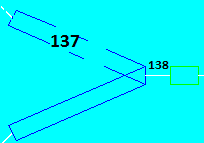
\includegraphics{fig8_ets.PNG}
  \caption{From reverse to forward propagation.}
  \label{fig:min:plus}
\end{marginfigure}
%
%

On \fref{min:plus} is displayed an actual run of \PTC\ using Forest's  Windows$^\text{\textregistered}$ interface. The magnets and drifts in dashed lines have reverse propagators. By looking at \fref{accel.fig8}, where the full Figure-Eight is displayed, the reader can easily spot magnet 137 and drift 138. In this case, the planes are perfectly aligned and, it would appear as in the LHC anecdote, that one does not need a patch. However the $x$-direction of 137 points downwards while on the drift 138 it points upwards. 

\PTC\ puts two patching rotations in this case. The first one is only used when connecting fibres with different directions of propagation; the information is at \lref{bx1:m}. Geometrically it is a rotation of 180 degrees around the $x$-axis. It inverts the $y$ and the $z$ axes. In practice, only $y$ co\"ordonates are inverted since the $z$ direction is not needed for propagation. However this maneuver leaves the $y$ axis pointing in the wrong direction, this is corrected by a \emph{bona fide} phase space rotation around the $z$ axis as shown on \lref{mu:pi}.

It is important to realize that this patch is computed with pure geometrical calculations using the exit frame of 137 and the entrance frame of 138.  The reader may wonder why \PTC 's patching routines did not select a rotation of $\pi $ around the $y$ axis. Rotations around the $x$ and $y$ axis are nonlinear drifts in polar co\"ordinates: they do not make any sense for angles beyond $\pi \over 2$ (See Eq.~\eqref{prot}). Therefore the decomposition of \PTC , while not unique, is necessary.



\makeussubscript
\endinput


